\chapter{Исскуство, Музыка, Художники}

\section{Дадаизм: история, основы и суть}

\textit{Источник: \url{https://4brain.ru/blog/dadaizm-istoriya-osnovy-i-sut/}}

Группа молодых людей дружно хохотала, сидя за столиком маленького кафе и обсуждая политику, африканскую музыку, скульптуру и \ex{ударные}{drums, percussion}. Все они сбежали от войны в эту нейтральную страну, чтобы жить, \ex{творить}{to create} и радоваться. И это не Дубай наших дней, а Цюрих вековой давности. В Первую мировую войну в его переулках родилось течение дадаистов, которые открыли новую главу в культуре Запада. Они научили людей думать и чувствовать по-другому.

\textbf{История дадаизма.}
Дадаизм \ed{многолик}{многоликий}{multifaceted, many-sided}. В этом стиле творили десятки, сотни людей в самых разных странах Европы и Америки. Каждый из них \ex{внес свою лепту}{made his contribution} в течение, но это же и стало его проклятием: т.к. у движения не было лидера, после завершения Первой мировой войны дадаисты разъехались по всему миру, от Японии до США, и стали творчески \ex{переосмысливать идеи}{to rethink ideas}, зародившиеся в Цюрихе.

У \ed{истоков}{исток}{место, где начинается водный источник (река, ручей); начало, первоисточник чего-н. («истоки первобытной культуры»)} дадаизма стоял немецкий поэт Хуго Балль. Изначально он поддерживал военню риторику и даже пытался вступить в армию добровольцем. Однако, когда Германия вторглась в Бельгию, Балль перестал поддерживать правящий режим, был назван родной страной предателем, поэтому был вынужден бежать туда, где говорили на его родном немецком языке: в швейцарский Цюрих. С собой Балль прихватил возлюбленную Эмму Хеннингс, которая также была поэтессой, и твердое убеждение, что война --- это зло.

\ex{Осев}{From the verb осесть: to settle} на берегах Цюрихского озера, влюбленные познакомились с владельцем винного погребка Meierei на улице Шпигельгассе. Он был очарован молодой парой, их \ed{задором}{задор}{enthusiasm} и творческой энергией. Предприниматель прикинул, что если сдаст им один из пустующих залов (совсем маленький, площадью около десяти квадратных метров), то сможет увеличить доходы с продажи пива многочисленным молодым собутыльникам Хуго и Эммы.

Расчет оправдался: владелец-голландец получил свои \ed{барыш\'{и}}{барыш}{\textit{устар.}, \textit{разг.} прибыль, материальная выгода}, а влюбленные --- место, которое они превратили в легендарное «Кабаре Вольтер». Сегодня мы бы назвали это место баром или кафе. Однако название было звучным и всем понравилось. Имя философа-просветителя 18 века влюбленные выбрали из-за написанной им повести «Кандид», в которой Вольтер \ed{высмеивал}{высмеивать/высмеять}{подвергать насмешкам, представлять в смешном виде; осмеивать (to make fun of; to mock; to ridicule)} религиозные и философские догмы своего времени.

Хуго и Эмму такой подход восхищал и вдохновлял. Они не остановились на религии и философии и за те долгие годы, что по миру грохотала Первая мировая война, \ex{переосмыслили}{rethought} догмы Старого Света, дав пищу искусству Нового Света (Америки) и послевоенной Европы.

Первое представление в «Кабаре Вольтер» состоялось 5 февраля 1916 года: молодежь организовала варьете с песнями на французском и немецком языке, русской и африканской музыкой, а также небольшую выставку.

Представление имело огромный успех. Круг общения Хуго и Эммы \ex{ширился}{expanded}, в него вливались все новые и новые эмигранты из европейских стран. Местных было очень мало. «Швейцарская молодежь слишком осторожна для кабаре», --- таково было мнение Хуго.

Хотя в мире \ex{бушевала}{was raging} Первая мировая война, эмигранты не голодали, иногда они ели стейки, запивали их хорошим испанским вином и праздновали подобающим образом. Молодые люди зарабатывали пером, игрой на пианино в пабах, рисовали для богатых заказчиков и выполняли другие частные заказы творческого характера.

Как и предсказывал хозяин Meierei, представления «Кабаре Вольтер» пользовались популярностью у населявших в тот момент Цюрих молодых людей, а потому приносили хорошие деньги.

14 июля 1916 года Балль выпустил основополагающий «Манифест Дада». Именно он определил \textit{вектор направления} дадаизма.

Откуда взялось его название, до конца непонятно. По одной версии, это славянское двойное утверждение (русское «да-да»). По другой, это детская игрушечная лошадка на французском языке. Существует с десяток других версий. Как истинные \ed{творц\'{ы}}{твор\'{е}ц}{creator}, дадаисты \ex{выступали за}{advocated for} плюрализм мнений.

\textbf{Лица дадаизма.} Балль оказался не только талантливым организатором, но и поэтом-новатором. В Европе его считают одним из создателей так называемой «фонетической поэзии». Он писал строки наподобие:

\begin{fancyquotes}
    «Gadji beri bimba glandridi laula lonni cadori\\
    gadjama gramma berida bimbala glandri galassassa laulitalomini\\
    gadji beri bin blassa glassala laula lonni cadorsu sassala bim».
\end{fancyquotes}


Эти слова никак не переводятся. Балль изобрел каждое из них. Это «стихи без слов». В строках нет смысла, но в этом и вся прелесть. Носителю славянских языков эти строки покажутся \ed{белибердой}{белиберда}{\textit{разг.}, \textit{пренебр.} что-либо нестоящее, несуразное, глупое; вздор, бессмыслица}, а европейцу --- чем-то прекрасным. Поэма будет иметь огромный успех в западной культуре и в 21 веке, когда дадаистам посвятят очередной Ноттинг-Хиллский карнавал.

«Сколько слов и словосочетаний можно вытащить из этого калейдоскопа? Это зависит от того, на какие языки и диалекты мы можем ссылаться (и является ли «Нонсенс» одним из них). Как на карнавале, где на каждом углу \ex{соперничают}{compete} многочисленные оркестры и звуковые системы, \ed{зевакам}{зевака}{тот (та), кто из праздного любопытства засматривается на кого-либо или рассматривает что-либо  (onlooker)} приходится постоянно \ex{настраивать}{tune} свои внутренние наушники.

Вы можете уловить в этих строках немного латыни, греческого, итальянского, румынского, шведского (возможно), турецкого, немецкого (конечно) и английского, --- и подозревать, что вы все еще прочесываете только верхушку айсберга», --- так охарактеризовала эти строки Балля его современная коллега из Великобритании Кароль Руменс [The Guardian, 2009].

Ближайшим соратником Хуго по кружку дадаистов стал выросший в Румынии артист Тристан Тцара. Он родился в еврейской семье под именем Самуэль Розеншток, а евреям в Королевстве Румыния не полагались полные гражданские права. Когда началась война, Самуэль порвал с родиной и стал творить на чужбине на французском языке. Именно Тцара выпустит вторую часть «Манифеста Дада» и продолжит дело Хуго, когда тот женится на Эмме и отойдет от дел «Кабаре Вольтер».

Значительный вклад в стиль дадаизма внесли скульпторы Марсель Янко и Жан Арп.

Особняком стоял французский художник Марсель Дюшан, который вместе с Пабло Пикассо и Анри Матиссом определит революционные разработки в пластическом искусстве 20 века. \ed{Пририсовать}{пририсовать}{нарисовать в дополнение к чему-либо уже нарисованному} «Моне Лизе» усики и бородку? Очень в стиле Дюшана. Сегодня это творение выставлено на почетном месте в парижском Центре Помпиду (Рис \ref{fig:mona-lisa})
\begin{figure}
    \centering
    \includegraphics[width=0.7\textwidth]{img/pompidou.jpg}
    \caption{Mona Lisa}\label{fig:mona-lisa}
\end{figure}


Поддержку дадаистам выражали:
\begin{enumerate}
    \item Цюрихский врач для бедных, социалист Фриц Брупбахер.
    \item Директор цюрихской школы имени Иоганна Генриха Песталоцци, галерист Хан Корай. Именно он предоставил дадаистам свою галерею в отличном месте, в доме Шпрюнгли, для выставок, мероприятий и крупных фестивалей «Дада».
    \item Анархист Юлиус Хойбергер разрешит дадаистам пользоваться своей типографией. Т.к. многие работы дадаистов были сложными по графике, хороший результат требовал сотрудничества издателя и творца.
    \item Местная пресса. Хотя во многих странах молодых дадаистов представляют как аморальных пьяниц, швейцарские журналисты того времени в целом относились к движению «Дада» с пониманием и уважением. «Редакция одного из ведущих швейцарских СМИ, которое с успехом переживет 20 век, Neue Zürcher Zeitung, и вовсе выражала дадаистам свою \ex{благосклонность}{отношение с симпатией, участием к кому-либо}», --- подчеркивают их коллеги из швейцарского журнала Schweizer Monat, который выходит в Цюрихе с 1921 года [B. Ruetz, 2003].
\end{enumerate}

С «Кабаре Вольтер» сотрудничали: (i) Василий Кандинский, (ii) Амедео Модильяни, (iii) Пабло Пикассо, (iv) Гийом Аполлинер, (v) Филиппо Томмазо Маринетти.

Само «кабаре» на улице Шпигельгассе просуществует недолго, всего полгода: открывшись зимой 1916 году, уже осенью того года его не станет. Дадаистов развелось так много, что им стало банально тесно на десяти квадратных метрах. Последний перфоманс «Кабаре Вольтер» пройдет летом 1916 года. В 1917 году была открыта Галерея Дада.

\textbf{Протест искусства или искусство протеста?}
Дадаизм – сын Первой мировой войны. Дадаизм в искусстве возник из разочарования миром, который допустил войну.

Многие дадаисты считали, что «разум» и «логика» буржуазного капиталистического общества привели людей к войне. Они выражали свое неприятие этой идеологии в художественном выражении, которое, казалось, \ex{отвергало логику}{rejected logic} и принимало хаос и иррациональность. Например, немецкий карикатурист Джордж Гросс позже вспоминал, что его дадаистские творения были задуманы как протест «против этого мира взаимного уничтожения».

Для дадаизма характерно противостояние позитивизму, научному мышлению, основанному на понятии разума, а также литературным и художественным традициям, чистоте \ed{отвлеченных понятий}{отвлеченное понятие}{abstract concept}.

Поэтому дадаизм исходил из необходимости порвать с устоявшимися тенденциями и способствовать анархии в художественном мире, даже навязывая идеологию и новый образ жизни, в которых отвергались традиционное и условное.

Немецкий художник Ханс Рихтер и вовсе утверждал, что дадаизм не был искусством: он был «антиискусством».

Дадаизм представлял собой противоположность всему, что символизировало искусство. Там, где искусство было связано с традиционной эстетикой, дадаисты игнорировали эстетику. Если искусство должно было воздействовать на чувства, то дадаизм должен был оскорбить.

Кроме того, стиль «Дада» попытался отразить человеческое восприятие и хаотичную природу общества.

Как выразился Балль: «Для нас искусство не \ex{самоцель}{end in itself}... но это возможность для истинного восприятия и критики времени, в котором мы живем» [Национальная галерея искусства в Вашингтоне, 2006].

С точки зрения дадаистов, массовое искусство и культура их времени представляли собой фетишизацию, когда объекты потребления (включая организованные системы мысли, такие как философия и мораль) выбираются так же, как торт или сорт вишни, чтобы заполнить пустоту.

\textbf{Характеристики и основы дадаизма.}
Дадаизм и искусство дадаизма не определяли единого стиля, поскольку основывались именно на критике традиционного чувства искусства, школы или стиля. Тем не менее, направление дадаизма объединено рядом общих принципов, придававших ему характерный тон как в литературном, так и в пластическом плане:
\begin{enumerate}
    \item \textit{Междисциплинарный характер}. Практически никто из дадаистов не творил только в одном жанре. Тот же Балль, помимо поэзии, был успешным журналистом, эссеистом, драматургом. Именно дадаисты придумали объединить фотографию и скульптуру.
    \item \textit{Отвращение концепции красоты}. Для дадаистов традиционная концепция искусства потеряла смысл перед лицом реальности насилия, развязанного в Европе. Молодые люди считали, что искать красоту и \ex{ублажать чувства}{satisfy the senses} недопустимо перед лицом ужасов войны.
    \item \textit{Антихудожественный и антилитературный смысл}. Т.к. дадаизм позиционировал себя как «антиискусство», для его понимания больше важны не формы, а концепция, способ воздействия на реальность.
    \item \textit{Оценка художественного жеста выше художественного объекта}. Дадаисты верили, что художник перестанет быть тем, кто рисует или ваяет, тем, кто творит красоту, и станет тем, кто выбирает предмет без эстетических претензий и придает ему смысл уже в самом факте своего выбора. Таким образом устанавливается эпоха, в которой жест художника будет действительно считаться «художественным».
    \item \textit{Ироничный, провокационный и дерзкий юмор}. Дадаизм предложил \ex{свирепое}{ferocious} издевательство над искусством --- не только традиционным искусством, но и авангардным искусством, таким как кубизм и футуризм (последний прославлял войну).
    \item \textit{Острая критика западного общества}. Предложение «Дада» построено как отказ от буржуазных ценностей начала века: слепой и \ed{бездумной}{бездумный}{thoughtless} веры в научно-техническое развитие как смысл истории, радикального национализма, культа капитала и использования искусства как транквилизатора совести.
    \item \textit{Заявление об иррациональности как отказ от позитивизма}. Поняв, что человеческий разум принес с собой не лучшую жизнь, а массовые разрушения, дадаисты стали настаивать, что искусство и литература больше не должны оправдываться именем разума. Таким образом, они возвели в приоритет иррациональность и абсурд. Этот способ работы сделал возможным беспрецедентное творческое развитие, хотя и не был свободен от споров и неприятий.
    \item \textit{Создание новых художественных техник}. Дадаисты популяризировали каллиграфию Аполлинера и созданный кубистами коллаж, изобрели фотомонтаж и реди-мейд (создание предмета искусства из повседневного объекта, например, \ed{писсуара}{писсу\'{а}р}{urinal}).
    \item \textit{Инновационное использование слова}. Привязанный к ценностям движения, дадаизм предпочитал использование слов по очереди, не будучи связанным очевидным значением или логическим дискурсивным смыслом. В качестве исходного материала они также брали сами буквы и звуки, что позволяло избежать ассоциации с рациональным смыслом. Важную роль в этом сыграла случайность.
\end{enumerate}
Дадаизм --- это не столько художественный жанр, сколько образ жизни. Молодые творцы ценили спонтанность, импровизацию, отказ от традиций. Причем, везде. В том числе в музеях. Именно они первыми стали использовать мусор в искусстве.

Дадаисты отказывались творить и думать по шаблону и учили этому других. Их эксперименты так вдохновят Запад, что «разрыв шаблона» станет устойчивым выражением у западных людей и даст начало популярной ныне теории когнитивного диссонанса. Если вы думаете, что это одно и то же, но сомневаетесь и хотите знать точно, как достичь консонанса, записывайтесь на нашу онлайн-программу «Когнитивистика».

Дадаисты обожали:
провокации,
\ex{эпатаж}{shocking},
демонстрации,
перфомансы,
скандалы,
фантастику,
экспрессию,
\ex{несовершенство}{imperfection},
естественность.

Поэтому в своей отрицательной строгости дадаизм выступал против модернизма и различных авангардных течений: экспрессионизма, кубизма, футуризма и абстракционизма, обвиняя их, в конечном счете, в том, что они являются заменителями того, что было уничтожено или вот-вот будет уничтожено.

Главный \ex{вклад}{contribution} дадаизма в современное искусство заключается в том, что дадаисты поставили вопрос о том, что такое искусство или что такое поэзия, привели людей к пониманию того, что все есть условность, которую можно подвергнуть сомнению, и, следовательно, не существует фиксированных и вечных правил, исторически узаконивающих художественное. Многое из того, что является провокационным в современном искусстве (например, смешение жанров и материалов, типичное для коллажа), происходит из дадаизма.

Хотя дадаисты использовали революционные методы, их идеи были основаны на глубокой вере, восходящей к романтической традиции, в присущую человечеству доброту, пока та не была испорчена обществом.

\textbf{География послевоенного дадаизма.}
Возникнув в Швейцарии в 1916 году в «Кабаре Вольтер», где был обнародован первый «Манифест Дада», дадаизм распространился по всей планете. После того, как Первая мировая война закончилась, цюрихские дадаисты разъехались по миру. Дадаизм в искусстве стал исключительно городским феноменом.


\textit{Дадаизм в Германии.}
5 июня 1920 года в Берлине прошла Международная ярмарка Дада. Центральной фигурой выставки стала свисающая с потолка фигура немецкого офицера с головой свиньи (Рис. \ref{fig:damaism-germany}).

\begin{figure}[h]
    \centering
    \includegraphics[width=0.8\textwidth]{img/dadaism-germany.jpg}
    \caption{Дадаизм в Германии}\label{fig:damaism-germany}
\end{figure}

Помимо перфомансов и прочего творчества, переехавших в послевоенную Германию дадаистов живо интересовала политика. Идеологически позиции художников-дадаистов были коммунистическими, а в некоторых случаях и анархистскими. Дадаисты занимали \ed{устойчивый левый сектор}{?}.

Дадаизм окончательно пустит корни в Германии, когда местный поэт Рихард Хюльзенбек выпустит немецкий манифест ДаДа и начнет издавать «Альманах Дада». До своей смерти в 1974 году Хюльзенбек будет повторять, что «ДаДа еще жив».

Именно немецкие дадаисты придумают использовать технику фотомонтажа и коллажа, чтобы запечатлеть окружающую их действительность, используя визуальный материал, взятый из СМИ.

\textit{Дадаизм в США.}
Европейские беженцы Дюшан, Пикабиа, Мина Лой и Жан Кротти вместе с американскими артистами Ман Рэем, Беатрис Вуд, Мортоном Шамбергом, Эльзой фон Фрейтаг-Лорингховен, Флориной Стеттхаймер дадут жизнь нью-йоркскому дадаизму.

Американские дадаисты \ed{примкнут}{примыкать/примкнуть + к чему-то}{to join} к авангардным течениям, которые \ex{назревали}{were brewing} в Гарлеме, Гринвич-Виллидж и Чайнатауне с начала века.

\textit{Дадаизм во Франции.}
Париж стал новым центром дадаизма в 1920 году.

Вдохновленные Тристаном Тцарой, французские дадаисты издавали манифесты, организовали демонстрации, ставили спектакли и выпускали журналы в стиле дадаизма.

В 1921 году дадаисты представят парижской публике свои работы в рамках Салона Независимых. Пьеса «Газовое сердце» Тцары вызовет бурю \ed{насмешек}{насмешка}{обидная шутка, издёвка}, а затем и целый театральный \ex{бунт}{riot}, который станет началом конца французского движения дадаизм. Сюрреализм --- это его \ex{детище}{то, что создано собственными трудами и заботами}, которое вырастет на \ed{осколках}{осколок}{fragment} парижского дадаизма.

Ураган дадаизма пронесется по Италии, Японии, Нидерландам, Югославии, Грузии, но Россию не затронет. В молодом советском государстве появится множество сочувствующих дадаизму лиц, однако официально советских творцов к направлению дадаизма не причисляют.

\textit{Космополитизм.}
Как и Сократ с Диогеном, дадаисты много размышляли над свободой отдельного человека и тем, что интересы личности и человечества в целом выше интересов отдельной страны. Европейские дадаисты были искренне уверены, что Западу пора кончать считать себя центром Вселенной, особенно в разгар \ed{бушующей}{бушующий}{raging} войны.

Дадаисты много общались с этнографами, археологами, историками, фольклористами. Музыка и песни дадаистов заимствовали ритмы и костюмы из Африки и Новой Зеландии, которую до прибытия европейцев населял народ маори.

Пытаясь отрицать, а в идеале, низвергнуть западную цивилизацию, дадаисты призывали вернуться к исцеляющим первобытным состояниям, не особенно волнуясь над степенью идеализации этих самых состояний.

Именно здесь оказалась зарыта «культурная бомба». В 21 веке во многих странах «примитивистские» выступления дадаистов считаются оскорбительными. Как и многие современные художники, принявшие «примитивизм», дадаисты присваивали незападные культурные артефакты, не понимая и не признавая их первоначальных ценностей и целей. Они предполагали, что африканские культуры и народы нерациональны, и стремились обобщить все африканские и океанические культуры в единое однородное целое [Khan Academy, Ch. Cramer, K. Grant, 2023].

И хотя дадаисты не стали мировыми знаменитостями, как импрессионисты или философы Древней Греции, они вошли в историю благодаря тому \ed{дерзкому}{дерзкий}{brazen, impudent, impertinent, insolent, cheeky, old, daring} вызову, что бросили цивилизованному миру. Их идеи пережили их самих, повлияв на мышление людей в самых разных странах, не только в Европе. Дадаизм 20 века --- это не столько про искусство, сколько про человека и его возможности. Именно поэтому дадаизмом так вдохновлялись такие гении 20 века, как Дэвид Боуи и Фрэнк Заппа, пропагандировавший самообразование.

Если вы тоже, как дадаисты, уже подошли к той мысли, что не все в этой жизни обусловлено разумом и логикой, и готовы идти по этой опасной дороге правды до конца, какой бы трудной и непредсказуемой она ни была, нам лишь остается пожелать вам \ed{стойкости}{стойкость}{firmness, steadfastness, staunchness, stableness} и храбрости на этом пути.


\newpage
\section{Художники}
\subsection{Виктор Михайлович Васнецов}
% https://muzei-mira.com/biografia_hudojnikov/765-viktor-mihaylovich-vasnecov-biografiya.html
В\'{и}ктор Мих\'{а}йлович Васнец\'{о}в родился в 1848 году 15 мая в селе со смешным названием Лопьял. Отец Васнецова был священником, также как и его дед и прадед. В 1850 году Михаил Васильевич увёз семью в село Рябово. Это было связано с его службой. У Виктора Васнецова было 5 братьев, один из которых также стал знаменитым художников, звали его Аполлинарий.

Талант Васнецова проявился с детства, но крайне неудачное \explainDetail{денежное}{д\'{е}нежный/-ая/-ое}{monetary} положение в семье не оставило вариантов, как отдать Виктора в Вятское духовное училище в 1858 году. Уже в 14-летнем возрасте Виктор Васнецов учился в Вятской духовной семинарии. Детей священников туда брали бесплатно.

Так и не окончив семинарию, в 1867 году Васнецов отправился в Петербург поступать в Академию художеств. Денег у него было совсем мало, и Виктор выставил на «аукцион» 2 свои картины -- «Молочница» и «Жница». До \explainDetail{отъезда}{отъезд}{departure} он так и не получил за них денег. 60 рублей за эти две картины он получил спустя несколько месяцев уже в Петербурге. \explainDetail{Прибыв}{прибывать/прибыть}{arrive} в столицу, у молодого художника было всего 10 рублей.

Васнецов отлично справился с экзаменом по рисованию и сразу \explain{был зачислен}{was enrolled (зачисл\'{я}ть/зач\'{и}слить: to enrol, to enlist)} в Академию. Около года он занимался в Рисовальной школе, где и познакомился со своим учителем -- И. Крамским.

К занятиям в Академии художеств Васнецов приступил в 1868 году. В это время он \explain{сдружился с}{made friends with} Репиным, и даже одно время они жили на одной квартире.

Хоть Васнецову и нравилось в Академии, но он её не закончил, уехав в Париж в 1876 году, где прожил больше года. В это время там же находился и Репин в \explainDetail{командировке}{командировка}{business trip}. Они также поддерживали дружеские отношения.

После возвращения в Москву Васнецова сразу приняли в Товарищество передвижных художественных выставок. К этому времени стиль рисования художника значительно меняется, да и не только стиль, сам Васнецов перебирается жить в Москву, где сближается с Третьяковым и Мамонтовым. Именно в Москве Васнецов \explainDetail{раскрылся}{раскрыв\'{а}ться/раскр\'{ы}ться}{to open, uncover oneself, to come out}. Ему нравилось находиться в этом городе, он чувствовал себя легко и \explainDetail{выполнял}{выполн\'{я}ть/в\'{ы}полнить}{to perform, execute, carry out} различные творческие работы.

Более 10 лет Васнецов \explainDetail{оформлял}{оформл\'{я}ть/оф\'{о}рмить}{put into shape, form} Владимирский соб\'{о}р в Киеве. В этом ему помогал М. Нестеров. Именно после окончания этой работы, Васнецова можно по праву назвать великим русским иконописцем.

1899 год стал \explainDetail{пиком}{пик}{peak} популярности художника. На своей выставке Васнецов представил публике «Трёх богатырей».

После революции Васнецов стал жить уже не в России, а в СССР, что его серьёзно \explainDetail{угнетало}{угнетать}{opress, depress, despirit}. Люди \explainDetail{уничтожали}{уничтож\'{а}ть/уничт\'{о}жить}{to destroy, obliterate; уничтож\'{е}ние: destruction} его картины, \explainDetail{относились}{относ\'{и}ться + \textit{дат.}}{to treat} неуважительно к художнику. Но до конца своей жизни Виктор Михайлович был в\'{е}рен своему делу -- он рисовал. \explainDetail{\'{У}мер}{умирать/умереть}{умир\'{а}ю, умир\'{а}ешь, умир\'{а}ют; умр\'{у}, умрёшь, умр\'{у}т: to die} он 23 июля 1926 года в Москве, так и не закончив портрет своего друга и ученик\'{а} М. Нестерова.



\subsection{Лики России Виктора Васнецова}

17 января в Центральной районной библиотеке им. А. П. Чехова прошла интерактивная лекция «\explainDetail{Лики}{лик}{character (like in a book)} России Виктора Васнецова»

Виктор Васнецов был известным мастером бытовой и исторической живописи. Его картины \explain{приобретали}{acquired} коллекционеры Павел Третьяков и Савва Мамонтов. Полотн\'{о} Васнецова «Богатыри» стало одним из первых обращений к был\'{и}нному сюжету в истории русской ж\'{и}вописи. Кроме нап\'{и}сания картин, Васнецов делал иллюстрации к книгам, создавал эскизы архитект\'{у}рных \explainDetail{сооружений}{сооружение}{construction, building, erection} и расписывал хр\'{а}мы в разных городах России.

Родился Виктор Васнецов 15 мая 1848 года в Вятской губернии (сегодня --- Кировская область) в семье священника. Родители старались дать детям \explainDetail{разностороннее}{разносторонний}{many-sided, versatile} образование: читали им научные журналы, учили рисованию. Первыми работами Виктора Васнецова были пейзажи, сюжеты сельской жизни. Природа на его картинах во многом списана с вятских видов: \explain{изв\'{и}листые}{meandering} реки, холм\'{ы}, \explainDetail{густые}{густой}{thick, dense} \explainDetail{хвойные}{хвойный}{coniferous (adj.); хв\'{о}я: coniferous} леса.

В 1858 году Васнецов поступ\'{и}л в дух\'{о}вное училище, затем -- в семинарию. Он изучал \explainDetail{жити\'{я}}{жити\'{е}}{life of a saint} свят\'{ы}х, хронографы, летописные своды, \explainDetail{пр\'{и}тчи}{пр\'{и}тча}{parable}. Древнерусская литература зародила в художнике интерес к старин\'{е}.

В свободное от учёбы время Васнецов рисовал портреты горож\'{а}н, делал по памяти зарис\'{о}вки, помогал расписывать Вятский кафедральный собор. В 1867 году он проиллюстрировал книгу этнографа Николая Трапицина о пословицах. Позже художник опубликов\'{а}л свои рисунки \explain{отдельно}{separately} -- в альбоме «Русские \explainDetail{пословицы}{посл\'{о}вица}{proverb, saying, adage} и \explainDetail{поговорки}{поговорка}{посл\'{о}вица} в рисунках В.М. Васнецова». В годы учёбы живописец создал первые пол\'{о}тна «Жница» и «Молочница».

В 1867 году Виктор Васнецов бр\'{о}сил семинарию и уехал в Петербург. Зимой этого года он занимался живописью в школе своего друга -- художника Ивана Крамского, а спустя год, поступил в Петербургскую академию художеств.

В академии Васнецов получил две малые серебряные медали за уч\'{е}бные работы, а через два года ему \explainDetail{вручили}{вруч\'{а}ть/вруч\'{и}ть}{to hand over, to deliver, to present,  to entrust} Большую серебряную медаль за картину «Христос и Пилат перед народом». В это время художник рисовал иллюстрации к сказкам и литературно-педагогическим трудам Николая Столпянского -- «Народная азбука», «Солдатская азбука». Во время жизни в Петербурге Виктор Васнецов создавал пол\'{о}тна бытового жанра -- «\explainDetail{Н\'{и}щие}{н\'{и}щий}{beggar} певцы», «С квартиры на квартиру», «Рабочие с т\'{а}чками». В 1874 году живописец получил бронзовую медаль на Всемирной выставке в Лондоне за картины «Книжная лавка» и «Мальчик с бутылкой вина».

После окончания академии художник уехал с друзьями за гран\'{и}цу. Там прод\'{о}лжил писать, участвовал в выставках и салонах. В парижской \explainDetail{мастерск\'{о}й}{мастерск\'{а}я}{workshop} своего др\'{у}га Василия Поленова Васнецов \explainDetail{наброс\'{а}л}{набр\'{а}сывать/наброс\'{а}ть}{to sketch, to draw an outline (набр\'{о}сок: sketch)} эскиз картины «Богатыри» -- первого полотн\'{а} по мотивам русских былин.

Васнецов прожил за границей около года, в 1877 году вернулся в Москву. Здесь познакомился с коллекционером Павлом Третьяковым, часто бывал на музыкальных вечерах в его семье.

В московский период художник писал картины с сюжетами из истории и сказок Древней Руси. Одно из первых пол\'{о}тен - «После \explainDetail{побоища}{побоище}{carnage} Игоря Святославича с половцами» -  экспонировалось на VIII выставке \explainDetail{передвижников}{передв\'{и}жник}{wanderer}. Картину купил Павел Третьяков.

Познакомился Васнецов и с меценатом Саввой Мамонтовым, стал участником его Абрамцевского кр\'{у}жка. Мамонтов \explainDetail{предлож\'{и}л}{предлаг\'{а}ть/предлож\'{и}ть}{to offer, to propose, to suggest} художнику напис\'{а}ть три картины для интерьера управления Донецкой железной дороги. Так появились пол\'{о}тна «Битва скифов со славянами\footnote{Battle of the Scythians with the Slavs}», «Ковёр-самолёт», «Три царевны подземного царства». Однако чл\'{е}ны \explainDetail{правления}{правление}{reign} отказались от пол\'{о}тен со сказочными сюжетами. Картины выкупили Савва Мамонтов и его брат.

Виктор Васнецов много бывал в Абрамцеве в ус\'{а}дьбе мецената, писал портреты членов его семьи. \explainDetail{Окр\'{е}стности}{окр\'{е}стности}{surroundings} Абрамцева появились и на других картинах Васнецова: березовые \explainDetail{р\'{о}щи}{р\'{о}ща}{grove} и изв\'{и}листые р\'{е}чки, \explainDetail{овр\'{а}ги}{овр\'{а}г}{deep narrow valley} и пруды, поросшие осокой. Здесь в 1880 году художник напис\'{а}л «Алёнушку».

Виктор Васнецов пр\'{о}бовал себя и в архитектуре. Он с\'{о}здал эскизы для \explainDetail{постр\'{о}ек}{постр\'{о}ека}{construction} в усадьбе Мамонтовых, по рисункам Васнецова и Поленова в Абрамцеве построили церковь Сп\'{а}са Нерукотв\'{о}рного. Также художник нарисов\'{а}л эскизы собственного дома-мастерской, \explainDetail{особняк\'{а}}{особн\'{я}к}{mansion} Ивана Цветкова, главного фасада Третьяковской галереи в Лаврушинском переулке в Москве.

В начале 1885 года профессор Петербургского университета Адриан Прахов, один из учител\'{е}й Васнецова, предлож\'{и}л ему расписать \explain{только что построенный}{just/newly built} Владимирский собор в Киеве. Васнецов называл \explain{р\'{о}спись}{(\textit{ж.р.}) painting, mural} хр\'{а}ма главной работой своей жизни -- он \explainDetail{посвят\'{и}л}{посвящ\'{а}ть/посвят\'{и}ть}{devote, dedicate [посвящ\'{а}ю, -\'{а}ешь, -\'{а}ют; посвящ\'{у}, посвят\'{и}шь, посвят\'{я}т]} ей около 11 лет. Художник говорил: «Нет на Руси для русского художника \explain{свят\'{е}е}{holier $<$ свят\'{о}й: holy, sacred} и \explain{плодотворнее}{more fruitful (плодотв\'{о}рный)} дела, как украшение хр\'{а}ма». Во время работы Виктор Васнецов изучал памятники раннего христианства в Италии, фрески Софийского соб\'{о}ра в Киеве, использовал знания иконописи и храмового \explainDetail{зодчества}{з\'{о}дчество}{ (dated) architecture}, пол\'{у}ченные в семинарии.

Всего было с\'{о}здано около 400 эскизов, расписано св\'{ы}ше 2000 квадратных метров. Собор освятили в 1896 году \explain{в присутствии}{in the presence of} императора Николая I и его семьи. После Владимирского собора художник расписывал храмы в Петербурге, \explainDetail{Гусь-Хрустальном}{Гусь-Хрустальный}{town in Vladimir Oblast}, Дармштадте, Варшаве.

До конца жизни Виктор Васнецов продолжал пис\'{а}ть картины по мотивам сказок. В 1898 году он закончил полотн\'{о} «Богатыри», над которым работал 25 лет.

Виктор Васнецов \explainDetail{\'{у}мер}{умир\'{а}ть/умер\'{е}ть}{to die; past tense: умер\'{а}л/\'{у}мер} в своей мастерск\'{о}й в 1926 году. Художника похорон\'{и}ли на Введенском \explain{кл\'{а}дбище}{cemetery} в Лефортово.


\subsection{Василий Васильевич Кандинский}
% https://muzei-mira.com/biografia_hudojnikov/2022-vasiliy-vasilevich-kandinskiy.html
Знаменитый создатель легендарного «Синего \explainDetail{всадника}{всадник}{rider}» обратился к сфере искусств \explain{относительно}{relatively} поздно -- в возрасте около 30 лет, что не помешало ему достичь значительных высот, став одним из создателей абстракционизма, основателем многочисленных художественных \explainDetail{объединений}{объединение}{union} и педагогом в Высшей школе строительства и художественного конструирования, более известной как Баухаус.

Кандинский происход\'{и}л из оригинального купеческого сибирского рода, где \explain{прич\'{у}дливо}{bizarrely} смешалась кровь тунгусских князей с древнейшей \explain{родословной}{pedigree}, не менее старинного княжеского рода манси и каторжников, \explainDetail{с\'{о}сланных}{с\'{о}сланный}{exiled ($<$ ссыслать/сослать)} в Нерчинск за \explain{Бог весть}{God knows} какие \explainDetail{провинности}{провинность (женский род)}{delinquency, fault}.

В детстве будущего художника его семейство много путешествовало по Европе и территории России, а затем \explain{поселилось}{settled} в Одессе, которая тогда была третьим по \explain{значимости}{significance} городом Российской империи. В этом чудесном южном городе Василий закончил гимназию, а также получил музыкальное и художественное образование. Несмотря на \explain{несомненное}{undoubted} \explain{даров\'{а}ние}{gifting, endowment, ability} мальчика, родители \explain{пр\'{о}чили}{intend, predict} ему карьеру юриста, что он и воплотил в жизнь, \explain{учась}{learning} с \explainDetail{перерывами}{перерыв}{break} в Московском университете.

Однако настоящая жизнь Кандинского как художника начинается с выставки импрессионистского искусства в Москве 1895 года, где его в самое сердце \explainDetail{поразила}{поражать/поразить}{to amaze, affect, stagger, startle} работа Клода Моне.
В следующем году он уезжает в Мюнхен, где \explain{погружается}{sinks, dives, plunges} в среду экспрессионизма, но н\'{а}чало Первой Мировой войны прерывает его становление и он возвращается на родину. Но с Советской Россией ему не по пути, и Василий Васильевич в 1921 году навсегда покидает родные пенаты. Он уезжает в Германию, откуда через некоторое время вместе с женой бежит во Францию от нацистов, закрывших Баухаус и признающих только \explain{собственное}{own}, глубоко формализованное и статичное искусство. В принявшей его стране он получает гражданство, становится известным и живет всю свою оставшуюся жизнь.

За годы своего творчества Кандинский основал объедин\'{е}ние «Фал\'{а}нга», школу, \explainDetail{участвовал}{участвовать/поуч\'{а}ствовать}{participate} в «\explainDetail{Бубновом валете}{Бубновый валет}{Jack of diamonds}», затем \explainDetail{заложил}{закл\'{а}дывать/залож\'{и}ть}{to put, to lay, to place ( залож\'{и}ть стран\'{и}цу: to mark a page, to put in a bookmark); to lay the foundations of; } Новое мюнхенское художественное объединение, а позже -- и знаменитый «Синий всадник».

В начале своей художественной карьеры мастер работал в реалистичной и \explain{частично}{partialy} абстрактной манере, экспериментировал с формами и цветом, писал на стекле.

Начав преподавательскую деятельность, Кандинский \explain{вск\'{о}ре}{soon} стал видным теоретиком абстракционизма и Баухауса. Его самые известные \explainDetail{пол\'{о}тна}{полотн\'{о}}{linen, canvas} -- это «Москва», «Восток», «Колебание» и «Композиция», одн\'{а}ко их очень много и каждое из них имеет п\'{о}лное право называться настоящим шедевром. Его картины \explain{исключительно}{exceptionally, exclusively} интересно рассматривать, \explainDetail{возникает}{возник\'{а}ть/возн\'{и}кнуть}{to arise, to appear, to emerge, to originate, to spring up} \explain{ощущение}{sensation, feeling}, что с каждой точки зрения в них открывается что-то новое и необычное.

К сожалению, пришедшие к власти фашисты успели уничтожить множество работ Василия Васильевича, как и других талантливых мастеров, причисленных к категории «дегенеративного искусства». Но и оставшихся пол\'{о}тен нам достаточно, чтобы понимать, каким великим талантом был Кандинский. \explainDetail{Скончался}{скончаться}{to pass away} мастер в 1944 году в Нейи, \explainDetail{пр\'{и}городе}{пр\'{и}город}{suburb} Парижа.


\section{Произведения}
\subsection{Картина «Три Богатыря» ВМ Васнец\'{о}ва}
% https://muzei-mira.com/kartini_russkih_hudojnikov/1321-opisanie-kartiny-bogatyri-tri-bogatyrya-vasnecova-1898.html

\begin{wrapfigure}{l}{0.5\textwidth}
    \begin{center}
        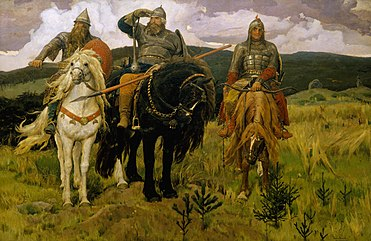
\includegraphics[width=0.49\textwidth]{img/tri_bogatyrya.jpg}
    \end{center}
    \caption{Картина «Три Богатыря» ВМ Васнец\'{о}ва (слева направо: Добрыня Никитич, Илья Муромец и Алёша Попович), ВикипедиЯ.}
\end{wrapfigure}
Картина В\'{и}ктора Мих\'{а}йловича Васнец\'{о}ва «Богатыр\'{и}» \explain{по пр\'{а}ву}{rightfully } считается настоящим народным \explainDetail{шед\'{е}вром}{шед\'{е}вр}{masterpiece} и с\'{и}мволом отечественного искусства. \explainDetail{Создав\'{а}лась}{создаваться/создаться}{create} картина во второй половине XIX века, когда среди русских художников был\'{а} очень популярна тема народной культуры, русского фольклора. Для многих художников это увлечение оказалось кратковременным, но у Васнецова народная фольклорная тематика \explainDetail{ст\'{а}ла}{стать/становиться}{become (ст\'{а}л/-а/-о)} \explainDetail{осн\'{о}вой}{осн\'{о}ва}{basis} всего \explainDetail{творчества}{творчество}{cretativity}.


На картине «\ed{Богатыр\'{и}}{богат\'{ы}рь}{A bogatyr or витязь is a stereotypical fictional character in medieval Russian legends}» \explainDetail{изображен\'{ы}}{изображён/-\'{а}/-\'{о}}{depicted; изображение: image, depiction; изображ\'{а}ть/изобраз\'{и}ть: to depict} три русских богатыр\'{я}: Илья Муромец, Добрыня Никитич и Алёша Попович -- знаменитые герои народных \explainDetail{был\'{и}н}{был\'{и}на}{epic}.

\explainDetail{Испол\'{и}нские}{испол\'{и}нский}{gigantic} фигуры богатыр\'{е}й и их коней, распол\'{о}женные \explain{на пер\'{е}днем пл\'{а}не}{in the foreground (пер\'{е}дний пл\'{а}н)} картины, символизируют силу и мощь русского народа. Этому \explainDetail{впечатлению}{впечатл\'{е}ние}{impression} \explainDetail{спос\'{о}бствуют}{способствовать/поспособствовать}{contribute to} и \explainDetail{внушительные}{внушительный}{impressive} размеры картины -- 295$\times$446 см.

Над созданием этой картины художник работал почти 30 лет. В 1871 году был с\'{о}здан первый \explain{набр\'{о}сок}{sketch} сюжета в карандаш\'{е}, и с тех пор художник увлёкся идеей создания этой картины. В 1876 году был сделан знаменитый \explain{эск\'{и}з}{sketch} с уже \explainDetail{н\'{а}йденной}{н\'{а}йденный/-ая/-ое}{$<$ найти} основой композиционного решения. Работа над самой картиной длилась с 1881 по 1898 год. Готовая картина была куплена П. Третьяковым, и до сих пор она \explainDetail{украш\'{а}ет}{украш\'{а}ть/укр\'{а}сить}{decorate} Государственную Третьяковскую галерею в Москве.


В центре картины изображён Илья Муромец, народный любимец, герой русских был\'{и}н. Не всем известно, что Илья Муромец не сказочный персонаж, а реальное историческое лицо. История его жизни и \explainDetail{р\'{а}тных}{р\'{а}тный}{military} \explainDetail{п\'{о}двигов}{п\'{о}двиг}{exploit, feat} -- это реальные события. \explain{Впосл\'{е}дствии}{subsequently}, закончив свои труды по охране родины, он стал монахом Киево-Печёрского монастыр\'{я}. Был причислен к л\'{и}ку свят\'{ы}х\footnote{was canonised}. Васнецов эти факты знал, создав\'{а}я образ Ильи Муромца. «\explainDetail{Матёр}{матёрый}{mature, fully grown, hardened} человек Илья Муромец» -- говорит былина. А на картине Васнецова мы видим могучего воина и при том \explainDetail{бесх\'{и}тростного}{бесх\'{и}тростный}{ingenuous, silly} открытого человека. В нём \explainDetail{сочетаются}{сочетаться}{combine} исполинская сила и \explain{великод\'{у}шие}{generosity, magnanimity, goodness}. «А конь под Ильёй \explain{лютый}{fierce} зверь» -- продолжает сказание. \explainDetail{Мощная}{мощный/-ая/-ое}{powerful} фигура коня, изображённого на картине с массивной металлической цепью вместо упряжки, \explainDetail{свид\'{е}тельствует}{свид\'{е}тельствовать}{testify; свидетель: witness} об этом.

Добрыня Никитич по народным преданиям был очень образ\'{о}ванным и \explainDetail{м\'{у}жественным}{м\'{у}жественный}{manly} человеком. С его личностью связано много чудес, наприм\'{е}р, заговорённая броня\footnote{charmed armor} на его плечах, \explain{волш\'{е}бный}{magic} меч-кладенец. Добрыня изображён таким как и в былинах -- величавым, с тонкими, благородными чертами лица, подчёркивающими его культурность, образ\'{о}ванность, \explain{решительно}{decisively} вынимающий меч из \explain{н\'{о}жен}{sheath} с готовностью \explainDetail{бр\'{о}ситься}{брос\'{а}ться/бр\'{о}ситься}{rush} в бой, защищая свою родину.

Алёша Попович \explain{по сравнению с}{as compared with} товарищами молод и строен. Он изображён с \explainDetail{л\'{у}ком}{лук}{bow} и стрелами в руках, но \explain{прикреплённые}{attached} к \explainDetail{седлу}{седло}{saddle} гусли свидетельствуют о том, что он не только бесстрашный воин, но и \explain{гусляр}{player of the musical instrument ``gusli''}, песенник, весельчак. В картине много таких деталей, которые характеризуют образы её персонажей.

Упряжки коней, одежда, амуниция не \explainDetail{вымышленные}{в\'{ы}мышленный/-ая/-ое}{imaginary, fictitious}. Такие образц\'{ы} художник видел в музеях и читал их описания в исторической литературе. Художник \explain{мастерски}{masterfully} передаёт состояние природы, как бы предвещающей о наступлении опасности. Но богатыри представляют собой \explainDetail{надёжную}{надёжный/-ая/-ое}{reliable} и мощную силу защитников родной земли.


\clearpage

\begin{wrapfigure}{l}{0.4\textwidth}
    \begin{center}
        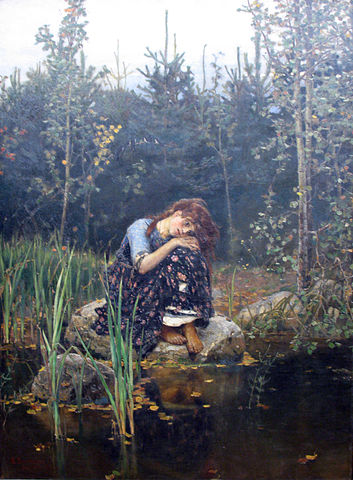
\includegraphics[width=0.38\textwidth]{img/alyonushka.jpg}
    \end{center}
    \caption{Алёнушка, ВикипедиЯ}
\end{wrapfigure}
\subsection{Картина «Алёнушка» ВМ Васнец\'{о}ва}
% https://muzei-mira.com/kartini_russkih_hudojnikov/1321-opisanie-kartiny-bogatyri-tri-bogatyrya-vasnecova-1898.html

Алёнушка, печальная девочка у \explainDetail{пруда}{пруд}{pond} --- одна из любимых всеми картин В. Васнецова. Художник уд\'{а}чно использует сказочный сюжет, чтобы \explainDetail{раскрыть}{раскрывать/раскрыть}{to open/to discover} сложный и неоднозначный русский характер.

Грусть девочки очень взрослая. Печаль в её глазах граничит с \explainDetail{отчаянием}{отч\'{а}яние}{despair}. Неубранные рыжие волосы, тёмные глаза, нежно-алые губы --- формируют легко читаемый образ ребёнка с тр\'{у}дной судьб\'{о}й.
В Алёнушке совсем нет ничего \explainDetail{сказочного}{сказочный}{fabulous, fairytale-like}, фантастического.
С\'{о}бственно, вся ск\'{а}зочность сюжета подчеркнута лишь одной деталью --- группой \explainDetail{ласточек}{л\'{а}сточка}{swallow}, сидящих над головой \explainDetail{героини}{героиня}{heroine}. Этим с\'{и}мволом (как известно, л\'{а}сточки символиз\'{и}руют над\'{е}жду) художник \explainDetail{уравновешивает}{уравновешивать/уравновесить}{to balance --- уравнов\'{е}шиваю/-ешь/-ют; уравнов\'{е}шу/-ишь/-ят} полный \explainDetail{тоск\'{и}}{тоск\'{а}}{yearning, longing} \'{о}браз героини, даёт надежду на счастливый финал старой русской сказки.

Васнецов нап\'{о}лнил \explain{ф\'{о}новый}{background} пейзаж атмосферой тишины и гр\'{у}сти.
Отлично удал\'{и}сь художнику в\'{о}дная \explain{гладь}{smooth surface} пруда, \explainDetail{камыш\'{и}}{камыш}{reed}, осока, \explainDetail{ели}{ель}{fir tree}.
Всё \explainDetail{неподв\'{и}жно}{неподв\'{и}жный/-ая/-ое}{still, motionless}, тихо, спокойно.
Даже пруд отраж\'{а}ет героиню очень деликатно, \explain{слегк\'{а}}{slightly}.
Чуть трепещут молодые \explainDetail{ос\'{и}ны}{ос\'{и}на}{aspen}. \explainDetail{Едва}{едв\'{а}}{barely, hardly} \explain{хмурится}{turns gloomly} ос\'{е}ннее небо.
Тёмные, зелёные тона пейзажа контрастируют с \explainDetail{румянцем}{румянец}{blush} на лице героини, а ос\'{е}нняя грусть --- с яркими цветами на юбке Алёнушки. Зритель чувствует: ещё мгнов\'{е}ние и сказка прод\'{о}лжится\dots







\subsection{Картина «Витязь на распутье»}

Виктор Михайлович Васнецов с циклом работ, \explain{посвященных}{dedicated (посвященный + \textit{дат.})} сюжетам русских сказок и былин, оказался \explainDetail{новатором}{новатор}{innovator} в этой области \explainDetail{изобразительного искусства}{изобраз\'{и}тельное искусство}{visual art}. За ним закрепилась репутация «художника-сказочника», он настолько проникся духом русской старины и былинного времени, что свой московский дом построил в виде деревянной избы (сейчас там находится мемориальный музей \explainDetail{живоп\'{и}сца}{живоп\'{и}сец}{painter, artist}).


Картина «В\'{и}тязь на расп\'{у}тье» \explain{отч\'{а}сти}{partly} является и отражением судьбы Васнецова.
Будучи \explainDetail{пр\'{и}знанным}{пр\'{и}знанный}{recognised} художником-передвижником, он, как и его товарищи, \explainDetail{исполнял}{исполнять/исполнить}{performed} жанровые композиции в духе остросоциальных тем, волновавших общество в 1870-1890-х.
Но завладевшая им сказочная тематика диктовала \explainDetail{ин\'{о}е}{ин\'{о}й/ин\'{а}я/ин\'{о}е}{(определительное местоимение) другой, отличный от данного; (неопределённое местоимение) некоторый. See \href{https://ru.wiktionary.org/wiki/\%D0\%B8\%D0\%BD\%D0\%BE\%D0\%B9}{wikictionary.org:иной}.} развитие творчества. Живописец уход\'{и}л от проблем современности и \explain{погружался}{plunge, dive} в мир русской старины, рискуя быть \explainDetail{осужденным}{осужденный}{convicted}.

\begin{wrapfigure}{l}{0.58\textwidth}
    \begin{center}
        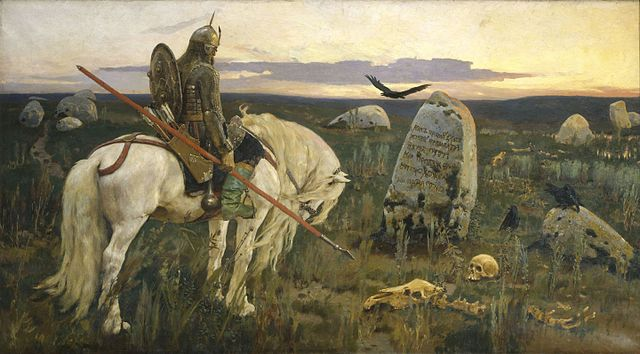
\includegraphics[width=0.57\textwidth]{img/TheKnightAtTheCrossroads.jpg}
    \end{center}
    \caption{Витязь на распутье, ВикипедиЯ}
\end{wrapfigure}
Выбор пути как один из \explain{роков\'{ы}х}{fatal} вопросов человеческой жизни на крупноформатном \explainDetail{холсте}{холст}{canvas} мастера приобрел эпическое звучание.
Перед камнем-предсказателем согнулся под тяжестью фатального \explainDetail{пророчества}{пророчество}{prophecy} опечаленный витязь. \explainDetail{Зловещий}{зловещий}{sinister} в\'{о}рон, садящееся красное солнце нагнетают\footnote{build up the atmosphere} атмосферу. \explainDetail{Нам\'{е}ренный}{нам\'{е}ренный}{intentional} отказ от \explainDetail{изображения}{изображение}{depiction} дороги (как выхода из трудности) художником сделан для того, чтобы показать \explain{неотврат\'{и}мость}{inevitability} судьбы.


\clearpage

% \chapter{Знаменитости}

\section{Пётр Налич}
Пётр Андреевич Налич (род. 30 апреля 1981, Москва) --- российский певец и композитор. Пишет песни, музыку к спектаклям, фильмам и мультфильмам.

В первый раз имя Петр Налич \explain{прозвучало}{звучать/прозвучать: to sound (here: was heard)} в 2007 году, когда Петр снял клип на свою песню «Гитар» и выложил её в интернет. Клип вошёл в ТОП-20 самых просматриваемых российских клипов русской версии ютьюба.

С 2008 года в составе МКПН (Музыкальный коллектив Петр\'{а} Налича) пел и \explain{сочинял}{сочинять/сочинить: to compose} песни в стиле, который сам характеризует как «весёлые бабури». \explain{Представил}{представлять/представить: (here) to introduce} Россию на конкурсе Евровидение 2010 как \explain{победитель}{winner} отб\'{о}ра, \explain{прошедшего}{прошедший: past participle of пройти, meaning ``past''} 7 марта 2010 года. Пётр Налич стал первым артистом в истории российской музыкальной индустрии, выпустившим в Интернете альбом («Радость простых мелодий») с использованием системы Pay What You Want («Заплати, сколько хочешь»)

\textbf{1981--2006: детство, юность.}
Пётр Налич родился в Москве в семье архит\'{е}кторов Андрея Захидовича и Валентины Марковны. Старший брат Павел --- художник-оформитель. По \explain{происхождению}{происхождение: origin (here: by origin)} --- дед по отцовской линии --- лирический тенор и диктор югославской редакции Московского радио (с 1993 года --- «Голос России»), Захид Омерович Налич был бошняком из города Тузла в Боснии и Герцеговине.

\begin{fancyquotes}
    Мой дед --- босниец. Был до войны лирическим тенором. Имел ангажемент в Белградской опере. Но потом война, лагерь, там ему фашисты \explain{гортань}{larynx} сломали, больше он не пел. Потом он попал в Советский Союз и здесь всю жизнь работал на радио
\end{fancyquotes}

Налич рассказывал, что его «папа \explain{част\'{е}нько}{quite often} пел за столом... Это и цыганские песни, и романсы». Пётр Налич окончил детскую музыкальную школу им. Мясковского, обучался в музыкальном училище при Московской консерватории им. П. И. Чайковского, а также в студии «Орфей» \explain{под руководством}{under the direction of} Ирины Мухиной. В 2010 году поступил в РАМ имени Гнесиных на специальность «Академическое пение» (класс проф. В. Левко). Среднее образование получил в школе No 1278. Пётр рассказывал, что в школе пел в хард-роковой группе: «Когда голос у меня сломался, стал громким, я стал петь с удовольствием. Вообще я всю жизнь пою. Я музыкальную школу закончил, играли в хард-рок в школе, потом в институте продолжил заниматься музыкой. Чуть позже начал заниматься вокалом и только тогда понял, что пою не очень хорошо».

\textbf{2006--2007: начало карьеры.}
Творчество Петр\'{а} Налича \explain{приобрел\'{о}}{приобретать/приобрести: to gain; to acquire}
известность после того, как он опубликовал на YouTube самостоятельно сделанный клип
на собственную песню «Гитар».
Клип был выложен весной 2007 года. А осенью, в течение одного месяца, клип посмотрело 70000 человек.
Ссылку на р\'{о}лик \explain{пересыл\'{а}ли}{пересылать/переслать: to forward}
друг другу пользователи Livejournal, число просмотров прирастало в день на тысячу. Затем в нескольких \explain{печатных}{печатный/печатные: printed} \explain{изданиях}{издание: publication} появились интервью с Петр\'{о}м и статьи о нём. \explain{Публика}{the public} \explain{потребовала}{требовать/потребовать: to demand} \explain{явления}{явление, the audience demanded the appearance of the artist} артиста.

У Петр\'{а} на тот момент было написано около 40 песен и музыкальных композиций, все они были выложены в свободном \explain{д\'{о}ступе}{д\'{о}ступ: access} на его сайте --- энтузиасты собрали из них архив, который до сих пор можно найти в интернете. Этот материал \explain{лёг}{ложиться/лечь: to lie down (past tense: лёг, легл\'{а}, легл\'{о}, легл\'{и})} в основу репертуара, с которым Пётр 9 ноября 2007 года дал свой первый концерт в клубе «Апшу».

Из-за ажиот\'{а}жа многие не смогли попасть \explain{внутрь}{same as внутри: inside} переполненного зрителями \explain{помещения}{помещение: premises}. Концерт прошёл успешно, появились статьи, \explain{\'{о}тзывы}{\'{о}тзыв: review} в блогах и прессе. Тогда Пётр собрал группу музыкантов и зимой 2008 года дал ещё два концерта в клубе «Икра». Билеты на эти концерты были раскуплены задолго до события. Группа получила название «Музыкальный коллектив Петр\'{а} Налича» (сокращённо МКПН).

\begin{fancyquotes}
    ``Гитар'' я сочинил года четыре тому назад, а клип записали этой весной. Снимали у меня на даче по Щелковскому шоссе. Мы просто тусовались, веселились. У нас там стояла убитая ``копейка'' друга моего брата, которую он никак не мог забрать. Все уже \explain{злились}{злиться: to get angry}, что она стоит на участке. Ну и решили её \explain{употребить}{употреблать/употребить: to use; to consume}, раз уж она здесь. \explain{Набились}{?} в неё все... ну, а дальше вы знаете.
\end{fancyquotes}

\textbf{2007---2010: первый альбом, участие в конкурсе «Евровидение».}
В течение двух следующих лет, помимо концертов в Москве, МКПН посетил с гастролями Петербург, Екатеринбург, Нижний Новгород и другие большие города России. Летом 2008 года МКПН поддерживал российские спортивные команды на Чемпионате Европы по футболу и Олимпиаде 2008 в Пекине. Затем коллектив выпустил свой первый альбом --- «Радость простых мелодий», фильм-концерт «МКПН в Б1 Maximum» и макси-сингл «Море». В 2009 году группа выступила хедлайнером на международном фестивале «Sfinks» в Антверпене.

7 марта 2010 года «Музыкальный коллектив Петр\'{а} Налича» с песней «Lost and Forgotten» был выбран в качестве участника от России на конкурс «Евровидение». Выступление на конкурсе в Осло принесло 11-е место.

\textbf{2010---2012: второй и третий альбомы}
6 апреля 2010 года прошёл первый концерт, на котором Пётр Налич исполнял не свои песни, а классический оперный репертуар и романсы. С тех пор подобные концерты проводятся регулярно. В 2010 году группа выпустила второй студийный альбом «Весёлые Бабури». Продажи стартовали 9 октября в клубе «Арена», а с 11 октября --- в музыкальных магазинах города.

С 2011 года Пётр Налич принимает участие в спектаклях театра-студии оперы РАМ имени Гнесиных под руководством проф. Ю. А. Сперанского. Спел партии Рудольфа в опере «Богема» Дж. Пуччини и Ленского в спектакле по опере П. И. Чайковского «Евгений Онегин».

Осенью 2012 года вышел третий альбом коллектива --- «Золотая рыбка».


\textbf{2013 год: четвёртый и пятый альбомы.}
В апреле 2013 года был выложен в сети четвёртый альбом --- «Песни о любви и родине», записанный Петр\'{о}м Наличем в сопровождении оркестра Ю. Башмета «Новая Россия» (дирижёр Игорь Разумовский). 17 мая 2013 состоялся концерт-презентация альбома в сопровождении оркестра «Новая Россия» в Светлановском зале ММДМ. Основу альбома составили новые композиции, никогда ранее не исполнявшиеся, написанные для вокала в сопровождении классического симфонического оркестра. В конце 2013 года выходит пятый альбом «Кухня», сборник эскизов (2005---2013) --- первый в мире альбом, записанный \explain{целик\'{о}м}{entirely} на языке бабурси. Некоторые композиции из этого альбома впервые были исполнены на новогоднем концерте в Известия-Холл, 29 декабря 2013 года.

\textbf{2014 год.}
22 апреля 2014 года Пётр, являясь артистом Театра-студии РАМ имени Гнесиных, исполнил партию Германа в опере П. И. Чайковского «\explain{П\'{и}ковая дама}{Queen of spades}» в Государственном музее А. С. Пушкина (режиссёр-постановщик --- заслуженный деятель искусств России, профессор Ю. А. Сперанский, режиссёр --- профессор Е. Бабичева)

Также, весной 2014 года МКПН выпустил макси-сингл «Sugar lies», записанный на средства, собранные с помощью акционеров в системе краудфандинг на сайте Планета

3-4 октября 2014 года Пётр Налич принял участие в театрализованных онлайн-чтениях «Каренина. Живое издание»

\textbf{2015 год.}
15 февраля 2015 года Пётр исполнил несколько песен из новой программы на конференции TEDxMoscow. 27 февраля 2015 в московском клубе «Известия-холл» была предст\'{а}влена новая программа «Песни сказочных героев», исполненная в сопровождении небольшого симфонического оркестра и х\'{о}ра (дирижёр Фёдор Сухарников, хормейстер Алия Мухаметгалиева). В неё вошли композиции из альбома «Песни о любви и родине», а также новые композиции, ранее не исполнявшиеся на публике. В течение 2015 года Пётр дал ещё несколько подобных концертов с этим коллективом в Москве, Санкт-Петербурге и Нижнем Новгороде.

Объявлено, что Музыкальный коллектив Петр\'{а} Налича находится в бессрочном творческом отпуске.

Пётр закончил обучение в РАМ им. Гнесиных по специальности «Академическое пение» \explain{с красным дипломом}{with honours}. В качестве дипломного спектакля спел партию Рудольфа («Богема» Пуччини) на сцене театра-студии оперы РАМ им. Гнесиных.

Осенью 2015 года в Российском Академическом Молодёжном Театре состоялась премьера спектакля «Северная Одиссея». Режиссёр --- Екатерина Гранитова. Художник --- Росита Рауд. Пластика, танцы --- Альбертс Албертс. Спектакль поставлен по киносценарию Петр\'{а} Луцыка и Алексея Саморядова. Музыку к спектаклю написал Пётр Налич, и сам же исполняет её на сцене вместе с коллективом музыкантов. 9 декабря 2015 состоялась презентация нового диска с саундтреком к спектаклю «Северная Одиссея».

Кроме того, 26 декабря в театре Вахтангова на малой сцене состоялась премьера детского спектакля «Питер Пэн», музыку для которого также написал Пётр. Режиссёр-хореограф --- Александр Коручеков. Сценография --- Максим Обрезков. Художник по костюмам и гриму --- Мария Данилова. Хореограф --- Сергей Землянский. Художник по свету --- Нарек Туманян. В спектакле также звучит музыка The Beatles, Queen, группы «АукцЫон».

\textbf{2016 год.}
2 февраля 2016 на сцене Пермского ТЮЗа \explain{состоялась премьера}{premiered} спектакля по пьесе Евгения Шварца «Обыкновенное чудо». Режиссёр спектакля Максим Соколов для работы над пьесой приглашает звездную команду: композитора Петр\'{а} Налича, хореографа Артура Ощепкова, художника-постановщика Валентину Серебрянникову. Премьерные спектакли собрали полные залы.

16 апреля 2016 года в ЦКМ НАУ в городе Киеве и 28 апреля в московском Театре Эстрады Пётр представил «неожиданный концерт-презентацию» под названием «Утёсов и не только...». Основную программу концерта составили песни из репертуара Леонида Утёсова. Петр\'{а} сопровождал большой эстрадно-симфонический бэнд под управлением Фёдора Сухарникова. Также на концертах был презентован диск «Утёсов», выпущенный к 120-летнему юбилею певца.

Осенью 2016 года был выпущен диск «Паровоз», записанный на средства, собранные с помощью акционеров в системе краудфандинг на сайте Планета. «Для меня особенно важно, что этот альбом записывается на деньги тех, кто хочет его услышать! Спасибо вам за это!», --- отмечает в своем обращении к поклонникам Пётр. 3 ноября состоялся концерт-презентация в Театре Эстрады. Пётр Налич выступил в сопровождении небольшого эстрадно-симфонического оркестра и хора. Одной из особенностей нового альбома стало то, что все песни и композиции сочинены специально для эстрадно-симфонического оркестра.

Следует отметить, что начиная с 2016 года состав музыкантов кардинально меняется, как и исполняемая Петр\'{о}м музыка. Формируется коллектив, куда приглашаются музыканты, уровень профессионализма которых соответствует новым сложным ритмам и мелодиям. Первым знаковым в этом смысле полноценным концертом стал концерт в Клубе 16 тонн, 10 декабря 2016 года. Презентация бэндовой программы с доработанными эскизами из альбома «Кухня». Пётр Налич und da Bande. --- премьеры: Аэроплан, Gasquerigym dym, Woodwind, Get ma Ola, Dead Husband. Вокал --- Пётр Налич; Хор: Геннадий Ивлев, Анфиса Затонская, Ильфат Баязитов, Мария Григорьева; Музыканты: Алиса Мандрик --- клавиши; Лев Слепнер --- перкуссии; Олег Маряхин --- баритон-саксофон, сопрано-саксофон; Антон Залетаев --- тенор-саксофон, флейта, блок-флейта; Павел Бокий --- труба; Ирина Бокий --- альт-саксофон; Дмитрий Сланский --- барабаны; Сергей Сокулер --- бас-гитара; Сергей Коньков --- гитара.

Продолжается сотрудничество с Оперным театром-студией им. Ю. А. Сперанского. 21 ноября 2016 года Пётр впервые исполняет партию Тамино в опере Моцарта «Волшебная флейта» в постановке Ольги Тимофеевны Ивановой.



\textbf{2017 год.}
17 мая 2017 года состоялся премьерный показ нового спектакля по одноименному рассказу А. П. Чехова «Тина» Академии кинематографического и театрального искусства Н. С. Михалкова на сцене Театрального зала Московского международного Дома музыки. Режиссёр дипломной постановки --- актёр, режиссёр, педагог Александр Коручеков. Сценография и костюмы --- Максим Обрезков. Композитор --- Пётр Налич.

1 октября 2017 года в Москве состоялась мировая премьера оперы-променад «Пиковая дама», в которой Пётр исполнил партию Германа. Классическая опера П. И. Чайковского впервые предстала в иммерсивном формате. Музыку Петр\'{а} Чайковского дополнили произведения неоклассика Николы Мельникова.

Режиссёр --- Александр Легчаков, хореограф --- Олег Глушков, художник-постановщик --- Полина Бахтина, дирижёр-постановщик --- Андрей Рейн.

\newpage
\section{Виктор Цой}
Виктор Робертович Цой (21 июня 1962 года, Ленинград --- 15 августа 1990 года, близ посёлка Кестерциемс, Латвийская ССР) --- советский рок-музыкант, автор песен и художник. Основатель и лидер рок-группы «Кино», в которой пел, играл на гитаре, писал музыку и стих\'{и}. Снялся в нескольких фильмах.

Виктор Цой родился единственным ребёнком в семье инженера корейского происхождения Роберта Максимовича Цоя и преподавательницы физкультуры Валентины Васильевны. Детство музыканта прошло в окрестностях Московского Парка Победы: он родился в \ed{роддоме}{роддом}{maternity hospital} на Кузнецовской улице (располагается внутри парка; сейчас это кардиоцентр), семья до 1990-х гг. жила в примечательном «генеральском доме» на углу Московского проспекта и улицы Бассейной (сейчас это памятник архитектуры). Некоторое время Виктор учился в \ed{близлежащей}{близлежащий}{(\textit{adj.}) nearby} школе на улице Фрунзе, где работала его мама. В 1973 г. родители Цоя развелись, а через год повторно вступили в брак.

С 1974 по 1977 год посещал среднюю художественную школу, где возникла группа «Палата No. 6» во главе с Максимом Пашковым.
После исключения за неуспеваемость из художественного училища имени В. Серова поступил в \explain{СГПТУ}{среднее государственное профессионально-техническое училище}--61 на специальность \ed{резчика по дереву}{р\'{е}зчик по дереву}{wood carver}.
В молодости был поклонником Михаила Боярского и Владимира Высоцкого, позднее Брюса Ли, имиджу которого начал подражать.
Увлекался восточными единоборствами и часто дрался «по-китайски» с Юрием Каспаряном.

\textbf{Смерть в автокатастрофе.}
15 августа 1990 года в 12 часов 28 минут Виктор Цой погиб в автокатастрофе. \explain{ДТП}{Дорожно-транспортное происшествие – это происшествие, при котором в результате движения по дороге или съезда с нее по крайней мере одного транспортного средства травмируется или погибает человек или наносится имущественный ущерб.} произошло на 35 километре трассы «Слока --- Талси» под Тукумсом в Латвии, в нескольких десятках километров от Риги. Согласно наиболее правдоподобной официальной версии, Цой заснул за рулём, после чего его «Москвич-2141» тёмно-синего цвета вылетел на встречную полосу и столкнулся с автобусом «Икарус» модели 250 (иногда этот автобус ошибочно идентифицируют как 280 модель.)

{\it Столкновение автомобиля «Москвич-2141» тёмно-синего цвета с рейсовым автобусом «Икарус-280» произошло в 12 час. 28 мин. 15 августа 1990 г. на 35 км трассы Слока --- Талси. Автомобиль двигался по трассе со скоростью не менее 130 км/ч, водитель Цой Виктор Робертович не справился с управлением. Смерть В. Р. Цоя наступила мгновенно, водитель автобуса не пострадал. ... В. Цой был абсолютно \ed{трезв}{трезвый}{sober} накануне гибели. Во всяком случае, он не употреблял алкоголь в течение последних 48 часов до смерти. Анализ клеток мозга свидетельствует о том, что он уснул за рулем, вероятно, от переутомления.

        --- из милицейского протокола; по данным сайта kinoman.net}

19 августа он был похоронен на Богословском кладбище в Ленинграде.

\textbf{Прочие версии гибели}.
Создатели документального кино из цикла «Следствие вели...» предположили, что Цой мог попасть в аварию, когда решил переставить другой стороной кассету в своём магнитофоне, тем самым отвлекшись от движения у «слепого поворота» дороги. Речь в передаче шла о кассете с демозаписью последнего альбома. Гитарист Юрий Каспарян ещё в 2002 году опроверг информацию о наличии этой кассеты в автомобиле Цоя: «Пользуясь случаем, хочу развеять миф, что на месте аварии нашли кассету с демо ``Черного альбома''... Все было не так. Я специально приехал в Юрмалу с аппаратурой, с инструментами и мы делали аранжировки для нового альбома. Когда доделали, я забрал кассету и поехал в Петербург. Я приехал утром, вечером узнал о случившемся. И поехал обратно. И кассета все время была у меня в кармане».


\textbf{Творчество.}
В конце 1970-х -- начале 1980-х началось тесное общение между Алексеем Рыбиным из хард-роковой группы «Пилигримы» и Виктором Цоем, игравшим на бас-гитаре в группе «Палата № 6», оба они познакомились в гостях у Андрея Панова (Свина), на квартире которого часто собирались компании, а также репетировала его собственная панк-группа «Автоматические удовлетворители».

Виктор Цой и Алексей Рыбин в составе «Автоматических удовлетворителей» ездили в Москву и играли панк-рок-металл на подпольных концертах Артемия Троицкого. Во время аналогичного выступления в Ленинграде по случаю юбилея Андрея Тропилло произошло первое знакомство с Борисом Гребенщиковым

\textbf{Первый альбом.}
Летом 1981 года Виктор Цой, Алексей Рыбин и Олег Валинский основали группу «Гарин и Гиперболоиды», которая уже осенью была принята в члены Ленинградского рок-клуба. \ed{Вск\'{о}ре}{вск\'{о}ре}{в недалёком будущем, через небольшой промежуток времени} Валинского забирают в армию, а группа, сменив название на «Кино», весной 1982 приступила к записи дебютного альбома. «Кино» под руководством Бориса Гребенщикова записывались на студии Андрея Тропилло в Доме Юного Техника, в записи принимали участие музыканты «Аквариума». Вскоре с ними же «Кино» дали свой первый электрический концерт в рок-клубе, всё выступление шло под драм-машину, а под песню «Когда-то ты был битником» из-за \ed{кулис}{кулиса}{backstage} на сцену \explain{выскочили}{jumped out} БГ, Майк и Панкер. К лету альбом был полностью завершён, продолжительность его звучания составляла 45 минут, откуда и появилось название. Но позже из окончательного варианта была убрана песня «Я --- асфальт», которую можно найти в переиздании «45», где она прилагается в качестве бонус-трека. \ed{Запись}{запись}{recording} получила некоторое распространение, о группе заговорили, начались квартирные концерты в Москве и Ленинграде. Вместе с будущим барабанщиком Зоопарка Валерием Кирилловым осенью этого же года «Кино» записывает в студии Андрея Кускова несколько песен, в том числе «Весна» и «Последний герой», вошедшие в сборник «Неизвестные песни Виктора Цоя» (всего четыре издания).

Тогда запись \explain{была забракована}{was rejected} и распространения не получила, так как Цой забрал ленту себе.

19 февраля 1983 года проходит совместный электрический концерт «Кино» и «Аквариума», музыканты выступали с тёмным макияжем и в костюмах со стразами. При этом они исполняли «Электричку», «Троллейбус» и «Алюминиевые огурцы». В основной состав был приглашён Юрий Каспарян. Весной из-за разногласий с Цоем Алексей Рыбин покидает группу «Кино». Лето уходит на совместные репетиции с новым гитаристом. В результате этого Виктор Цой и Юрий Каспарян записали альбом «46», который вначале задумывался как демозапись «Начальника Камчатки». Алексей Вишня «скинул» запись нескольким друзьям на плёнку. «46» получил широкое распространение и был воспринят как полноценный альбом. Осенью 1983 года Виктор Цой лёг на обследование в психиатрическую больницу на Пряжке, где провёл полтора месяца, избегая призыва в армию. После выписки из психиатрической клиники он пишет песню «Транквилизатор». Весной выступил на втором фестивале рок-клуба, где группа «Кино» получила лауреатское звание, а песня «Я объявляю свой дом безъядерной зоной», открывшая фестиваль, признана лучшей антивоенной песней фестиваля 1984 года.



\textbf{Второй состав «Кино».}
Летом 1984 года в студии «Антроп» Андрея Тропилло начинается запись альбома «Начальник Камчатки», к которому, кроме Виктора, приложили свою руку БГ и Сергей Курёхин.

В феврале 1984 Виктор и Марьяна празднуют свадьбу. На свадьбу были приглашены Гребенщиков, Майк, Титов, Каспарян, Гурьянов и другие.

Весной 1985 «Кино» заработали ещё одно звание лауреата и засели в студию к А. Тропилло писать «Ночь». Работа над записью затянулась из-за желания создать новую музыку с новыми приёмами игры. Альбом никак не получался, Виктор бросил «Ночь» недоделанной и в студии Алексея Вишни занялся записью «Это не любовь», который получился всего за неделю с небольшим. К осени «Это не любовь» была сведена и удачно разошлась по стране, а в январе 1986 вышла «Ночь», среди песен которой были известные «Мама Анархия» и «Видели ночь». Параллельно с выходом пластинки растёт популярность Виктора Цоя, а в феврале на 4-м фестивале рок-клуба «Кино» получает диплом за лучшие тексты. 5 августа 1985 года у Цоя родился сын Саша.


Летом 1986 года Виктор работал в бане на проспекте Ветеранов, он там мыл помещения из \ed{брандспойта}{брандспойт}{hose}. Необходимо было приходить на один час в день, но это было время с 22 до 23 часов, что ему мешало, так как Цой проводил это время суток с группой.

Также летом все участники группы уезжают в Киев на съёмки фильма «Конец каникул» (режиссёр Сергей Лысенко), а чуть позже дают совместный концерт с «Аквариумом» и «Алисой» в ДК МИИТ в Москве, с этими же группами в США выходит «Красная волна». Осенью Сергей Фирсов приглашает Виктора работать кочегаром. Цой соглашается, и они оба начинают работать кочегарами в котельной «Камчатка», откуда выросли многие знаменитые рок-музыканты.

В ней Рашид Нугманов организовал съёмки короткометражки «Йя-Хха», там же проходят съёмки фильма «Рок» Алексея Учителя --- оба фильма при участии Цоя. Осень и зима проходят в Ялте на съёмках «Ассы» Сергея Соловьёва.

Весна 1987 богата концертными событиями: премьера «Ассы» в ДК МЭЛЗ, последнее участие на фестивале рок-клуба, где «Кино» получили приз «За творческое совершеннолетие».

На порто-студии «Yamaha MT44» «Кино» начинают записывать альбом «Группа крови». Осенью 1987 года Виктор улетает к Рашиду Нугманову в Алма-Ату на съёмки своего последнего фильма «Игла», в связи с этим «Кино» доработали «Группу крови» и на время прекратили концертную деятельность. В 1988 выходит «Игла» и «Группа крови», которые породили «киноманию».

Начинаются триумфальные гастроли по Советскому Союзу --- «Кино» собирают аншлаги на всех концертах.

16 ноября 1988 на мемориальном концерте памяти Александра Башлачёва публика ведёт себя крайне активно; по плану концерт должна была заканчивать песня Башлачёва «Время колокольчиков» (в записи), памяти которого был посвящён концерт, но по невыясненным причинам во время выступления Цоя (он играл на гитаре) внезапно включили «Время колокольчиков», Цой прекратил играть, не понимая откуда идёт звук, который он не производит и что вообще происходит. Администрация многократно объявляла, что всем н\'{у}жно расходиться, концерт окончен. Цой не уходил, он несколько раз подходил к выключенным микрофонам и проверял, работают ли. Потом разводил руками --- «не работает», и ходил по сцене туда и сюда с цветком, не уходя со сцены, но и не имея возможности петь и что-то сказать публике. Публика не расходилась, люди шумели, кричали, было видно, что что-то идёт не так. Создавалось впечатление, что некая злая воля решила прекратить концерт и включила финальную песню прямо во время выступления Цоя. Через 10 минут этого противостояния администрация включила микрофон. Цой, в очередной раз подойдя проверять микрофон, услышал что он включён, и объявил людям, что по непонятным причинам несвоевременно была включена финальная песня Саши Башлачева, но после этого петь и играть уже не очень удобно. После этого он стал собираться и публика потянулась к выходу.

Весной 1988 записывается черновик, а зимой окончательный вариант альбома «Звезда по имени Солнце», который решили выпустить осенью. Цой знакомится с Юрием Айзеншписом, который с 1989 стал продюсером «Кино», организовывая концертные туры и частые выступления на телевидении, после чего группа обретает всесоюзную популярность. В день 50-летия Цоя Александр Градский в эфире канала «Москва-24» рассказал, что в тот период Артемий Троицкий инспирировал письмо в Московский Горком, которое должно было настроить московских рок-музыкантов против Виктора Цоя.

На телевидении Виктор Цой дебютировал в программе «Взгляд», об этом рассказано в книге «Взгляд» --- битлы перестройки.

В начале 1989 группа «Кино» впервые едет за границу во Францию, где выпускают альбом «Последний герой». Летом Виктор с Юрием Каспаряном едут в США. Тем временем «Игла» выходит на второе место в прокате советских фильмов, а на кинофестивале «Золотой Дюк» в Одессе Виктора Цоя признают лучшим актёром СССР.

24 июня 1990 года прошёл последний концерт «Кино» в Москве на Большой спортивной арене Лужников. На этом концерте, впервые после московской Олимпиады-80 был зажжён огонь в Олимпийской чаше. После этого Цой с Каспаряном уединились на даче под Юрмалой, где на порто-студию начали записывать материал для нового альбома. Этот альбом, дописанный и сведённый музыкантами группы «Кино» уже после смерти Цоя, вышел в январе 1991 и получил символическое название «Чёрный альбом», с соответствующим оформлением обложки.

\newpage
\section{Елена Ваенга}
Ел\'{е}на В\'{а}енга (настоящее имя --- Ел\'{е}на Влад\'{и}мировна Хрулёва; род. 27 января 1977, Североморск, Мурманская область, РСФСР, СССР) --- российская \explain{эстрадная певица}{pop singer}, автор песен, актриса. Лауреат премий «Шансон года».

В\'{а}енга --- это название родного для Елены Хрулёвой города Североморска до 18 апреля 1951 года, а также реки недалеко от него. В основе названия и псевдонима --- саамское слово «\explain{олен\'{и}ха}{deer}» (кильд. вайонгг). Псевдоним придуман её матерью.

\textbf{Биография.} Родилась 27 января 1977 года в Североморске. \explainDetail{Петь}{петь}{to sing} и \explain{обучаться}{to study (+ dative)} музыке начала с трёх лет.

Мать Елены Ваенги по образованию химик, отец --- инженер, работали в посёлке Вьюжный на \explain{судоремонтном заводе}{shipyard (судно: vessel; ship, plural: суда)} «Нерпа», который обслуживает атомные \explain{подводные лодки}{подводная лодка: submarine}. Про отца и родной Север у Елены Ваенги есть песня:

{\it У меня глаза северных цветов,\\
И мне не нужны тропические страны.\\
Я всегда с тобой рядышком была.\\
Жаль, что ты уехал слишком рано.\\
Я вдруг поняла: все эти города\\
Я должна пройти, как в наказанье.\\
Но у меня есть дом, а у дома --- я,\\
А у Севера --- сиянье}

Дед Елены со стороны матери --- контр-адмирал Северного флота Василий Семёнович Журавель, он упоминается в книге «Знаменитые люди Санкт-Петербурга». Бабушка Надежда Георгиевна Журавель (её крёстная) (род. 1927). Про неё у Елены Ваенги есть песня: «Моя бабушка любит суши...». Родители отца --- \explain{коренные}{коренн\'{о}й ж\'{и}тель; коренн\'{ы}е ж\'{и}тели: indigenous} петербуржцы, \explain{пережили}{(переживать/пережить) to survive; to experience} блокаду Ленинграда. Дед по линии отца --- зенитчик, во время \explain{Великой Отечественной войны}{second world war} \explainDetail{воевал}{воевать/повоевать}{to fight} под Ораниенбаумом, а бабушка по линии отца была врачом в госпитале в блокадном Ленинграде.

У Елены Ваенги есть младшая сестра Татьяна, она работает в дипломатической сфере, знает несколько языков.

Гражданский муж Елены Ваенги \explain{на протяжении 16 лет}{for 16 years} с 1995 по 2011 год --- Иван Иванович Матвиенко (род. 1957) --- продюсер певицы, по национальности цыган, был женат, его дочь на 2 года старше Елены Ваенги, раньше Иван перегонял машины из Германии.

Племянник, Руслан Сулимовский --- директор её коллектива.

В ночь с пятницы на субботу 10 августа 2012 года Ваенга в родильном доме No. 16 Санкт-Петербурга родила сына Ивана. 30 сентября 2016 года Елена официально вышла замуж за Романа Садырбаева.

\textbf{Творческая \explain{деятельность}{activity}.} Первую песню «Голуби» написала в 9 лет, стала победительницей Всесоюзного конкурса молодых композиторов на Кольском полуострове. После школы приехала в Санкт-Петербург, где закончила музыкальное училище им. Н. А. Римского-Корсакова по классу фортепиано, получив диплом педагога-концертмейстера. Некоторое время преподавала музыку в школе. Факультативно занималась вокалом.

Елена Ваенга с детства мечтала стать актрисой, поэтому после музыкального училища поступила в Театральную академию (ЛГИТМИК) на курс Г. Тростянецкого, но проучилась лишь два месяца, так как её пригласили в Москву записывать первый альбом. Продюсером певицы стал Степан Разин. Под псевдонимом Нина она выпустила клип на песню «Длинные коридоры» (композиция была издана в 2011 году на сборнике «Живая струна»). Альбом был записан, но не вышел. Разочаровавшаяся в шоу-бизнесе певица сбежала от Разина и уехала в Санкт-Петербург. Тем временем её песни взяли в свой репертуар Александр Маршал («Невеста»), Татьяна Тишинская («А ты налей мне белого вина», «Мама, что ты плачешь», «Володенька», «Угостите даму сигаретой»), группы «Стрелки» («Тонкая веточка»), «Божья коровка» («Сердце моё», «Самая любимая моя») и другие известные исполнители. Эти песни распространил её бывший продюсер. Елена Ваенга приняла решение с ним не судиться.

В Санкт-Петербурге Ваенга узнала, что в Балтийском институте экологии, политики и права на кафедре театрального искусства набирает курс П. С. Вельяминов, и в 2000 году пошла учиться к нему. Закончив курс, получила диплом по специальности «драматическое искусство». Выступила в антрепризном спектакле «Свободная пара» в паре с однокурсником Андреем Родимовым (режиссёр Екатерина Шимилёва).

Концертирует с девятнадцати лет. Лауреат петербургского конкурса «Шлягер года 1998» с песней «Цыган», «Достойная песня 2002». Участник концертов-фестивалей «Весна романса» в БКЗ «Октябрьский», «Вольная песня над вольной Невой», «Невский бриз». Дала несколько сольных концертов в ДК имени М.Горького. Гастролирует по России и другим странам и каждый год, в конце января, даёт концерт в БКЗ «Октябрьский» по случаю своего дня рождения.

Настоящая популярность пришла к певице в 2005 году с выходом альбома «Белая птица», в котором было много хитов: «Желаю», «Аэропорт», «Тайга», «Шопен» и заглавная композиция, на которую вышел клип.

28 ноября 2009 года Елена Ваенга получила свой первый приз «Золотой граммофон» за песню «Курю».

4 декабря 2010 года Елена повторила свой успех, получив во второй раз премию «Золотой граммофон» за песню «Аэропорт». В том же году певица впервые стала лауреатом фестиваля «Песня года», исполнив композицию «Абсент». А 12 ноября она дала первый в своей концертной деятельности сольный концерт в Государственном Кремлёвском дворце, трансляция которого прошла на Первом канале 7 января 2011 года. В телеанонсе Елене Ваенга была дана следующая характеристика:
Елена Ваенга --- тонкая, художественная, мечтательная и романтичная натура. Музыкальная одарённость, природный темперамент, трудолюбие, жизнерадостность --- всё это составляющие её жизни и творчества... Несмотря на внешнюю хрупкость и молодость, за спиной у этой очаровательной девушки богатая творческая биография и не такая уж простая человеческая судьба. Жанр, в котором работает певица, с большим трудом определяет даже она сама: «На 50 процентов это фолк-рок, есть старинные баллады, городские романсы, шансон. Но границы между ними провести почти невозможно.»
--- анонс на Первом канале --- «Белая птица». Концерт Елены Ваенги
В 2011 году Елена Ваенга приняла участие в ежегодной церемонии национальной премии Шансон года в Кремле, на которой исполнила песни «Оловянное сердце» и «Девочка». Популярность певицы растёт. В январе этого же года она победила Леонида Агутина в телепередаче «Музыкальный ринг» на канале НТВ, набрав почти в пять раз больше голосов слушателей.

26 ноября 2011 года певица в третий раз получила премию «Золотой граммофон» за песню «Клавиши», но на концерте в Кремле исполнила композицию «Шопен». 21 декабря 2011 года певица в третий раз дала концерт в Кремле. В 2012 году на «Золотой граммофон» претендовали песни «Шопен» и «Где была».

В 2011 году Елена Ваенга дала 150 афишных концертов, гастролировала в США, Германии, Израиле.

Периодически играет в спектакле «Свободная пара», совместно с Андреем Родимовым.

В 2011 году Ваенга впервые попала в список самых успешных деятелей российского шоу-бизнеса, составленный Forbes, и заняла в нём девятую позицию, с годовым доходом более шести миллионов долларов.

В репертуаре певицы --- собственные песни, старинные и современные романсы, баллады и народные песни, а также песни на стихи классиков, таких, как Сергей Есенин («Задымился вечер») и Николай Гумилёв («Жираф», «Шут»). В 2012 году певица провела концертный тур по Украине и Германии. Однако на этом деятельность певицы оборвалась в связи с потерей голоса из-за механического повреждения связок. После выздоровления певица дала последние концерты в городах Средней Волги и ушла в отпуск.

В ноябре 2012 года певица вышла из декрета и возобновила концертную деятельность. По сведениям журнала Forbes, в 2012 году певица в списке самых успешных российских деятелей шоу-бизнеса заняла четырнадцатое место. Сама артистка это отрицает, также как и в прошлом году, утверждая, что её доход гораздо меньше. На данный момент артистка активно гастролирует.

В 2014 году Елена Ваенга стала одним из членов жюри шоу Первого канала «Точь-в-точь».

27 ноября 2015 года состоялся сольный концерт Ваенги в Государственном Кремлёвском дворце, где она выпустила новую программу и представила новый альбом.


\section{Почему Джордж Майкл взял себе такой псевдоним?}

Настоящее имя британского певца Джорджа Майкла --- Йоргос (Георгиос) Кириакос Панайоту. В 1982 году молодой дуэт «Wham!», в составе которого он выступал, выпустил свой первый официальный сингл «Wham Rap!». На его обложке, помимо второго вокалиста Эндрю Риджли, красовалось имя Джордж Панос. Джордж --- это производное от Георгиос, а Панос --- фамилия отца поп-звезды, которую тот взял себе, эмигрировав из Греции в Великобританию в 1950-х годах. Он сменил имя Кириакос Панайоту на Джек Панос.

«Это было, когда я изменил своё имя. Я всегда знал, что мне придётся изменить его, но они уже начали выпуск ``Wham Rap!'', а я всё ещё не выбрал себе псевдонима. Так что около двадцати тысяч экземпляров того первого релиза вышли с моим настоящий именем на обложке: Джордж Панос. И на этом этапе я понимал, что должен буду выбрать что-нибудь», --- позже рассказал в своём интервью Джордж Майкл.

Однако покорять мировые чарты с именем Джордж Панос певцу не хотелось, и он решил придумать себе более яркий псевдоним. Ему всегда нравилось имя Майкл, так звали брата его отца и школьного приятеля, также имевшего греческие корни. Поэтому певец принял решение взять себе фамилию Майкл. Все последующие хиты певец исполнял под псевдонимом Джордж Майкл.

«Я подумал, что это было бы отличным псевдонимом. Оно легко произносилось, и я не должен был отказываться от своего греческого происхождения полностью. Я не забывал об этом, хотя большинство людей решили, что это было еврейским именем», --- рассказал Джордж Майкл.


\clearpage

\section{Кино}
\textbf{Возникновение\footnote{возникновение: emergence}.}
В конце XIX века движение предмета наконец-то \explain{удал\'{о}сь}{удаваться/удаться: to manage} \explain{перенести}{переносить/перенести: to transfer} на экран. Вскоре после этого, кино начало набирать популярность. Первые фильмы были очень короткие, продолжительностью около 1-ого минуты. Они были черно-белыми и без звука. \explain{Спуст\'{я}}{later; after; e.g., спустя три дня} несколько лет продолжительность фильма уже составляла 15-20 минут.

\textbf{Виды фильмов.}
Существует несколько видов фильмов, такие как короткометражное кино, документальные и художественные фильмы.
Короткометражное кино является \explain{отд\'{е}льным}{отд\'{е}льный: separate} жанром. Нужно быть профессионалом, чтобы передать целый ряд чувств за короткий промежуток времени. Продолжительность таких фильмов обычно не \explain{превышает}{превышать: to exceed} 15-20 минут.

В основе документальных фильмов лежат реальные истории и факты. Обычно, это фильмы об исторических \explain{событиях}{событие: event}, знаменитых людях и т.д.
Образовательные фильмы также относятся к этой категории.

Художественные фильмы --- это фильмы, в которых актёры играют определённую роль. Художественные фильмы бывают разного жанра: мелодрамы, комедии, триллеры и другие.

\textbf{Российское кино.}
Стремительное \explain{развитие}{development} российского кино началось в XXI веке. Многие фильмы \explain{напр\'{а}влены}{short form of направленный (adj.): directed} на массового зрителя и, \explain{в большинстве своем}{largely}, развлекательные. Кроме того, \explain{выпускается}{выпускаться/выпуститься: to be released} большое количество фильмов высокого качества. Российский кинематограф известен своими талантливыми режиссёрами, такими как Никита Михалков, Федор Бондарчук, Тимур Бекмамбетов и некоторыми другими.

\textbf{Голливуд.}
Голливуд является самым популярным местом по \explain{производству}{производство: production} фильмов в мире. Ежегодно там \explain{создаются}{создаваться/создаться: to be created} тысячи фильмов. Голливудские фильмы полны спецэффектов, которые привлекают миллионы людей в кинотеатры.

\section{Человечество решает умереть}
\textit{Ярослав Забалуев}\\
\url{https://lenta.ru/articles/2021/12/25/dontlookup/}

{\it Вышла комедия про дураков и апокалипсис с Ди Каприо, Стрип и Бланшетт. Зачем ее смотреть?}

\textit{На Netflix вышла новая комедия известного «Игрой на понижение» Адама Маккея «Не смотрите наверх» --- хвастающая, возможно, самым звездным за последнее время актерским составом. «Лента.ру» рассказывает, почему фильм о конце света с Леонардо Ди Каприо в главной роли --- идеальное кино для конца этого странного года.}

Астрономы Рэндалл Минди (Леонардо Ди Каприо) и Кейт Дибиаски (Дженнифер Лоуренс) обнаруживают, что к Земле мчится комета диаметром в десяток километров. Столкновение с планетой может привести к полному исчезновению не только человеческой, но и вообще всякой жизни. Рэндалл и Кейт грузятся в самолет и отправляются в Вашингтон, чтобы обсудить планы спасения Земли с высочайшими государственными чинами. Однако выясняется, что президент Дженни Орлин (Мэрил Стрип) куда больше увлечена живописным курением и секстингом с каким-то региональным отморозком. Главой администрации работает ее сын Джейсон (Джона Хилл), который в свою очередь в основном хвастается новой татуировкой дракона и упивается властью ходить на работу упоротым.

Минди и Дибиаски пытаются добиться огласки, выступив в популярном телешоу, однако Кейт заслуживает лишь волну мемов в интернете, а Рэндалл --- недвусмысленные знаки внимания ведущей (Кейт Бланшетт), которую возбуждает, что скоро мы все умрем. В какой-то момент правительство США все же снарядит спасательную экспедицию, но сразу после старта развернет ракеты, поскольку на сцену выйдет Питер Ишервелл (Марк Рейланс) --- визионер, объясняющий, что из столкновения с кометой тоже в теории можно извлечь пользу.

Фильмы и сериалы-катастрофы прошлого и нынешнего годов дали повод вновь заговорить о сверхъестественном чутье художников, прозревающих будущее без всяких на то логических объяснений. Вот и разработка «Не смотрите наверх» началась еще во вполне безмятежном ноябре 2019-го. Впрочем, никакой безмятежностью, разумеется, и не пахло --- Дональд Трамп вовсю собирался на второй срок, а Америка все глубже погружалась в депрессию, лекарство от которой так и не придумали до сих пор. Тем не менее за без малого полтора года, которые занял путь картины к зрителю, в мире изменилось слишком многое, создав для «Не смотрите наверх» уникальный и куда более подходящий случаю контекст.

В сверхъестественной проницательности в данном случае стоит обвинять сценариста и режиссера Адама Маккея. Это автор удивительной судьбы. Шесть лет назад он не пожелал сидеть в комедийном жанровом гетто и после дилогии про Рона Бургугди («Телеведущий») бросился покорять новые территории. В итоге его «Игра на понижение» стала одним из самых остроумных фильмов про кризис 2008-го года и принесла Маккею «Оскар» за лучший адаптированный сценарий. Через три года, в 2018-м, Адам решил развить успех и одновременно взвинтить ставки --- его «Власть» имела в своем центре ни много ни мало бывшего вице-президента Дика Чейни. Сатирический байопик абсолютного зла (именно такова трактовка Маккея) был воспринят чуть менее однозначно, несмотря на очередной актерский подвиг Кристиана Бейла. И вот в следующем своем проекте режиссер совместил едкий социальный комментарий с внешне легкомысленным задором своих ранних комедий.

\begin{fancyquotes}
    Кажется, что фильмы про летящие к Земле кометы вышли из моды на рубеже тысячелетий --- нулевые показали, что над нами летают штуки и пострашнее
\end{fancyquotes}

Последней из больших голливудских картин на тему, конечно, был пропагандистский шедевр Майкла Бэя «Армагеддон». Это было кино, где все важные вещи говорили на фоне развевающегося звездно-полосатого флага, а Брюс Уиллис, наконец, смог погибнуть --- но только под песню Aerosmith. Самым ярким послесловием к этому сюжету стала «Меланхолия» Ларса фон Триера, который с явным удовольствием разнес-таки нашу планету в труху. «Не смотрите наверх» отсылает к этим двум фильмам вполне прямолинейно. «Армагеддон» спародирован целыми фрагментами, а Уиллиса заменил Рон Перлман --- и так даже смешнее. С «Меланхолией» у Маккея значительно более нежные отношения. Пародиями тут не пахнет, скорее уж речь идет о трепетном оммаже --- при желании героинь Лоуренс и Бланшетт можно без особых поправок поместить в триеровский контекст.

Однако прямые и не очень аллюзии в данном случае отнюдь не самоцель. Маккей использует энергию предшественников, чтобы напитать ей совершенно авторское высказывание, сделанное, как водится, в сатирическом ключе. Режиссер владеет этим сложнейшим на самом деле жанром виртуозно и в «Не смотрите наверх» явно упивается возможностью не заботиться об исторической достоверности. На орехи тут достается абсолютно всем: озверевшим от самодовольства селебрити политикам, мямлям-ученым, не способным разговаривать человеческим языком, дурящим народ визионерам со своими дурацкими смартфонами… Перечислять мишени Маккея можно долго и с удовольствием, благо режиссер не придерживается более или менее никакой конкретной позиции --- просто стреляет во все, что видит.

За без малого два с половиной часа от такого потока желчи и презрения можно было бы устать, но фокус в том, что «Не смотрите наверх» этих потоков на зрителя, в общем, не льет. Остроумие наблюдений и сарказм авторских комментариев здесь уравновешен удивительно человечной интонацией. У Маккея с его врожденной язвительностью и острым глазом нет ответов на вопрос «что делать?» За происходящим на экране балаганом сквозит растерянность умного человека, вынужденного, как обычно, пытаться хоть как-то достучаться до идиотов. Это, пожалуй, и правда самая адекватная эмоция в мире, где ученый, сообщающий в ток-шоу о гибели человечества, добивается лишь статуса «астронома, которого я бы трахнула». Зато об этом мире можно снять фильм, который под конец очередного безумного года дарит не столько депрессию, сколько радость и умиротворение. Если мы все равно скоро умрем, то нет ни одной причины отказываться от праздничного ужина.

Фильм «Не смотрите наверх» (Don't Look Up) вышел на Netflix 24 декабря

\clearpage

% \chapter{Мода}

\section{Как мода влияет на нашу жизнь?}

\textit{Источник: \url{https://absurdu.net/fashion/kak-moda-vliyaet-na-nashu-zhizn.html}}

С развитием современных технологий, соцсетей и рекламы большинство из нас осознает, что в той или иной мере мы таки поддаемся определенным трендам и модным тенденциям. И все же, существует немало тех, кто категорически не согласен с этим утверждением. Такие люди утверждают, будто бы мода никоем образом не влияет на их жизнь и, тем более, на поведение. Но так ли это на самом деле? Давайте разбираться!

\textbf{Отражает мировые события и общий настрой людей.}
Ни для кого не секрет, что мода всегда отражает культурные, социальные, политические, экономические и религиозные аспекты общества. Если в мире происходит что-то масштабное, это в любом случае тем или иным образом повлияет на fashion-индустрию. Так формируются определенные тренды. Яркое доказательство этому – тенденции 2021 года. Психологи говорят о том, что при возникновении неприятных событий человек нуждается в том, что могло бы положительным образом повлиять на его настроение. Этот принцип находит свое отражение и в модной индустрии. После пандемии и локдауна многие чувствуют усталость и подавленность. Дизайнеры, ощущая потребности своих клиентов, начали создавать более комфортную, но в то же время креативную одежду: мода понемногу отходит от нейтральных оттенков и непрактичных вещей, наоборот, повседневные предметы гардероба становятся более удобными, а палитра цветов гораздо ярче. Насыщенные цвета радуги положительным образом влияют на наше самоощущение и восприятие мира, а интересные фасоны, асимметрия или архитектурный крой в одежде смотрятся нарядно и элегантно, что способствует ощущению воодушевленности и праздничного настроения.

К интересным выводам пришли также те, кто занимается изучением истории fashion-индустрии. После масштабных войн или экономических кризисов одежда становилась все более откровенной. Фасоны прилегали к телу, подолы юбок и платьев укорачивались. С одной стороны, это было связано с практичностью, а с другой – с банальной нехваткой материалов. Из-за тяжелого положения в такие времена люди просто не могли тратить по 40 метров ткани на одно платье!
То же самое можно сказать и про сферу религии и морали. Все знают, что в мусульманских странах девушки не могут носить одежду, которая бы открывала их шею, запястья или щиколотки. Поэтому мода в таких государствах обычно гораздо более консервативная, но все же поддается изменениям. Тем более, что под хиджабом или паранджей женщина может носить то, что нравится ей, если это соответствует принципам одежды, записанным в Коране. Кроме того, в большинстве случаев они не ограничены в выборе аксессуаров. Так, например, во всемирно известном торговом центре Dubai Mall в ОАЭ, куда съезжаются люди из всех уголков мира, довольно часто можно встретить пару, в которой супруга идет в лодочках от любимого люксового бренда, а руках у нее оригинальная сумка Chanel или Dior.

\textbf{Продвигает инклюзивность, меняет представление о красоте.}
Конечно, представление о «красоте» очень субъективное, но, тем не менее, наше восприятие этого абстрактного понятия в огромной мере зависит именно от «канонов» fashion-индустрии. До 70-80-х прошлого века люди не сильно обращали внимание, на то, как выглядит их тело. Но с популяризацией спорта и развитием некоторых его видов в моду приходит «культ тела», подразумевающий подтянутую спортивную фигуру не только у мужчин, но также и у женщин. Вспомните также, как менялось представление об идеальных модельных параметрах: в 2000-е годы большинство представительниц этой профессии имели явно нездоровый вид, что чаще всего было следствием анорексии. Со временем, когда суровый fashion-мир наконец-то переосмыслил понятие красоты и здоровья, на подиумы стали выходить модели плюс-сайз. То же самое касается и темнокожих девушек: еще в конце прошлого века для большинства из них принять участие в показе или появиться на обложке глянца казалось недостижимой целью, а сегодня вопрос происхождения не является препятствием при построении карьеры. Если говорить об особенностях, как, например, кожа супермодели Винни Харлоу или страбизм (косоглазие) Брунетт Моффи, все больше людей также перестают обращать на это внимание.

Выпускники Лондонского колледжа моды Джудит Ахумба-Велленстайн, Сьюзан Джин и Пак Лунчиу, которые создали онлайн-журнал Hajinsky, посвященный фэшн-психологии, изучив то, какое воздействие мода имеет на жизнь большинства людей, пришли к следующему выводу:

\begin{fancyquotes}
    «Официальная одежда положительно влияет на абстрактное мышление человека, которое связано с такими действиями, как, например, экономия денег. Кроме того, наука показала, как бренды могут улучшить жизнь общества, сделав одежду инклюзивной. Исследования показали, что люди с ограниченными физическими возможностями часто для удобства носят спортивные костюмы и поэтому подвергаются двойной дискриминации — во-первых, из-за своей физических особенностей, во-вторых, из-за своей одежды. Бренды, принимающие это во внимание, могут в корне изменить жизнь человека».
\end{fancyquotes}

\textbf{Исполняет роль идентификатора личности.}
Мода также помогает нам больше понять других и служит неким идентификатором. Например, по национальному костюму мы можем догадаться, из какой страны человек, общий внешний вид иногда указывает на род деятельности, а характерная манера сочетать вещи может служить неким маркером «творчества», «вкуса» и т.д. Те же, кто все еще категорически отказываются принимать факт влияния моды на их жизнь, не могут отрицать того, что в современном мире просто нельзя избежать ситуаций, когда мы должны выглядеть определенным образом. Представьте, что вас пригласили на свадьбу, на торжественный ужин в дорогой ресторан или же вы идете на собеседование в крупное финансовое учреждение с наличием определенного дресс-кода. Для такой ситуации вы вряд ли наденете джинсы. Для подобных случаев существует различные наряды, в том числе классический деловой костюм, который так же пришел в нашу жизнь под влиянием определенных тенденций. Нельзя отрицать тот факт, что внешний вид человека также сказывается на том, как другие воспринимают его. Именно по этой причине мы часто задумываемся о том, какую одежду подбирать не только под определенную ситуацию, но даже под сам круг общения. Наше естественное желание нравиться способствует тому, что время от времени мы обновляем свой гардероб и добавляем туда красивые (которые соответствуют нашему субъективному вкусу) предметы одежды и аксессуаров.

\begin{fancyquotes}
    «Реальность такова, что мода стала частью нашей повседневной жизни. Она связана с политикой и может вызвать социальные перемеФормирует сознаниены. Мода также влияет на наши отношения друг с другом, наше поведение, она может улучшить нашу жизнь, помогая с самоидентификацией»,- заявили вышеупомянутые основатели журнала Hajinsky.
\end{fancyquotes}

\textbf{Формирует сознание.}
И это касается даже тех, кто никогда не следит за ней. Если все начинают носить оверсайз, со временем при покупке новой футболки вы также сделаете выбор в пользу прямого или более свободного фасона. Кроме того, это отражается и в количестве покупаемых предметов. Сейчас большинство людей приобретают намного больше одежды, обуви и аксессуаров, чем это было еще 30 лет назад.

\begin{fancyquotes}
    «При выборе гардероба важно ориентироваться на свои ценности и цели. При этом человек не может существовать в полном отрыве от общества. В этом смысле, если „психология моды“ про гармонизацию запросов общества и внутренних процессов человека, то это может повысить качество его жизни». – Говорит психолог Александра Меньшикова.
\end{fancyquotes}

Также нельзя забывать, что мода – это не только об одежде. Поэтому если вы не следуете трендам при формировании своего гардероба, это не значит, что вы не изучите последние тенденции, когда, например, будете делать ремонт в квартире. То же самое касается приобретения новой техники, автомобиля или даже посуды на кухню.

Хотите вы того или нет, мода в любом случае влияет на ваш выбор повседневных образов, домашней обстановки и даже места для отдыха. И это нельзя определить как «хорошо» или «плохо» — каждый оценивает по-своему. Остается лишь принять тот факт, что мода в большой степени влияет на разные сферы нашей жизни, а вот активно следовать новым тенденциям, принимать их или всеми силами пытаться убежать от них – личное дело каждого. Но, согласитесь, знание — сила. Осознанность поможет вам разумно подходить к вопросу трендов и тенденций, чтобы умело использовать этот инструмент для достижения своих целей. Актуальный и стильный внешний вид еще никому не помешал.